\chapter{TAkka: Evaluation}
\label{takka_evaluation}

\begin{center}
(This chapter is expanded from the companion paper, Chapter 6, 7 and 8)
\end{center}
\vspace{12 pt}

This chapter evaluates the TAkka library with regards to the following three 
aspects.  Firstly, Section~\ref{type_pollution} shows that the notion of 
type-parameterized actor in the TAkka library has syntactical advantages to 
avoid type pollution problem.  Secondly, Sections 
\ref{expressiveness} to \ref{efficiency} show that rewriting Akka programs 
using TAkka will {\it not} bring obvious code-size and runtime overheads. 
 Thirdly, Section~\ref{reliability} gives two accessory libraries, ChaosMonkey 
and SupervisionView, for testing the reliability and availability of TAkka 
applications. 



\section{The Type Pollution Problem}
\label{type_pollution}

In a system with multiple components, different components may require
different interfaces; since all messages are received in the same
mailbox, a naive approach would be to set the type to the union of all
the interfaces, causing each component to see a type containing
messages not intended for it---an issue dubbed the Type Pollution
Problem.

This section illustrates the Type Pollution Problem and its solution on an
instance of the Model-View-Controller pattern \citep{reenskaug1979original, burbeck87}.  The Model
and View have separate interfaces to the Controller, and neither
should see the interface used by the other.  However, the naive
approach would have the Controller message type contain all the
messages the Controller receives, from both the Model and the View.
A similar problem can occur in a multi-tier architecture \citep{fowler2002patterns},
where an intermediary layer interfaces with both the layer above
and the layer below.

One solution to the type pollution problem is using separate channels
for distinct parties.  For instance, in Model-View-Controller, one
channel would communicate between Model and Controller, and a distinct
channel communicate between Model and View.  Programming models that
support this solution includes the join-calculus \citep{full_join} and
the typed $\pi$-calculus \citep{pi_book}.  Can we gain similar
advantages for a system based on actors rather than channels?

The TAkka solution is publishing a component as of different types to different 
parties.  The published type shall be a supertype of the most precise type of 
the component.  In Java and Scala applications, this solution can be tricky 
because, as will be briefly discussed in Section~\ref{type_pollution_oo}, a set 
of supertypes must be defined in advance.  
Fortunately, if the component is implemented as a type-parameterized actor, 
the limitation can be avoided straightforwardly.  The demonstration example 
studied in this section is a Tic-Tac-Toe game with a graphical user interface 
(GUI) implemented using the MVC pattern.


\subsection{Case Study: Tic-Tac-Toe}


\subsubsection{The Game}

Tic-Tac-Toe \citep{wiki:tictactoe}, also known as Noughts and Crosses, is a 
paper-and-pencil game.  A basic version of the Tic-Tac-Toe game is played by 
two players who mark X and O in turn in a $3\times3$ grid.  A player wins the 
game if he or she succeeds in placing three respective marks, i.e. three Xs or three Os, in a 
horizontal, vertical, or diagonal row.  The game is drawn if no player wins when 
the grid is fully marked.

Figure~\ref{tictactoe_example} gives an example game won by the first player, 
X.  Figures \ref{fig:t0} to \ref{fig:t7}  are screenshots 
of the game implemented in the next subsection.  The graphical user interface 
of the game contains three parts.  The left hand side of the window shows the 
player with the next move.  The middle of the window shows the current status of 
the game board.  The right hand side contains control buttons, each of which 
kills one component of the application and test if that component will be 
restarted.  Finally, Figure~\ref{fig:t8} announces the winner.

\begin{figure}[p]
     \begin{center}
        \subfloat[]{
            \label{fig:t0}
            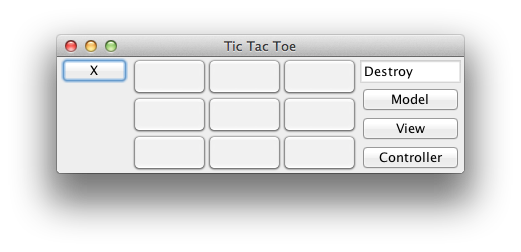
\includegraphics[scale=0.38]{TicTacToeScreenCut/0.png}
        }
        \subfloat[]{
           \label{fig:t1}
           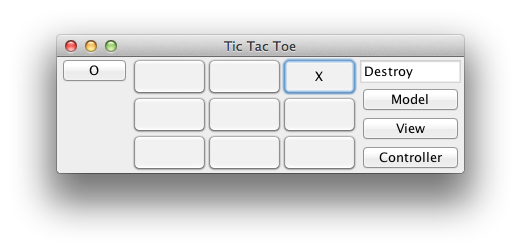
\includegraphics[scale=0.38]{TicTacToeScreenCut/1.png}
        }\\
        \subfloat[]{
            \label{fig:t2}
            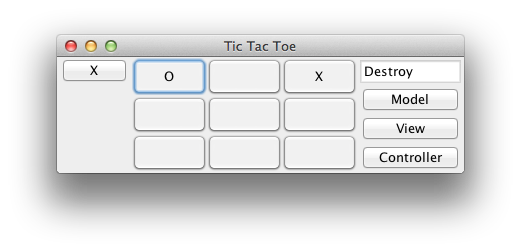
\includegraphics[scale=0.38]{TicTacToeScreenCut/2.png}
        }
        \subfloat[]{
            \label{fig:t3}
            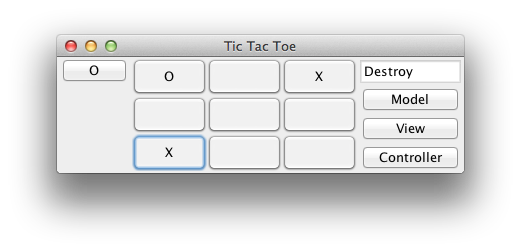
\includegraphics[scale=0.38]{TicTacToeScreenCut/3.png}
        }\\
        \subfloat[]{
            \label{fig:t4}
            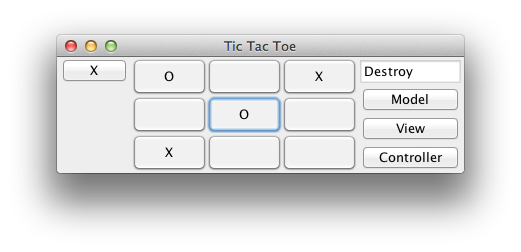
\includegraphics[scale=0.38]{TicTacToeScreenCut/4.png}
        }
        \subfloat[]{
           \label{fig:t5}
           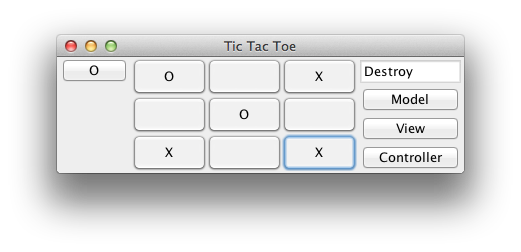
\includegraphics[scale=0.38]{TicTacToeScreenCut/5.png}
        }\\        
        \subfloat[]{
            \label{fig:t6}
            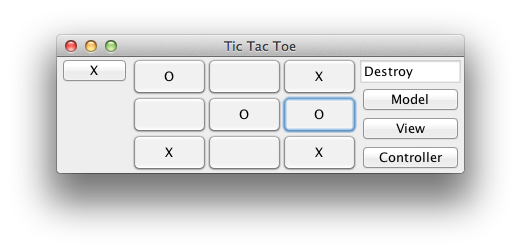
\includegraphics[scale=0.38]{TicTacToeScreenCut/6.png}
        }
        \subfloat[]{
           \label{fig:t7}
           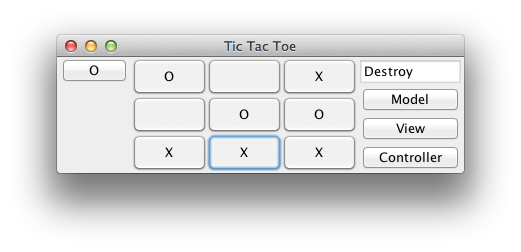
\includegraphics[scale=0.38]{TicTacToeScreenCut/7.png}
        }\\                
        \subfloat[]{
           \label{fig:t8}
           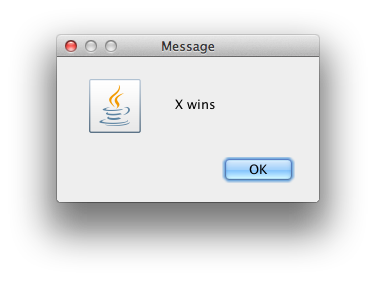
\includegraphics[scale=0.38]{TicTacToeScreenCut/8.png}
        }\\                        
    \end{center}
     \caption{A Game of Tic-Tac-Toe}
   \label{tictactoe_example}
\end{figure}


\subsubsection{The MVC pattern}

Model-view-controller (MVC) is a software architecture pattern introduced by 
\citet{reenskaug1979original}.  The pattern separates the data abstraction
(the model), the representation of data (the view), and the component for 
manipulating the data and interpreting user inputs (the controller).  
One key design principle of MVC is that the model and the view {\it never} 
communicate with each other directly.  Instead, the controller is responsible 
for coordinating the model and the view, for example,  sending instructions and 
reacting to messages from the model and the view.  

MVC has been widely used in the design of applications with a graphical user 
interface (GUI), from early Smalltalk programs written in Xerox Parc 
\citep{reenskaug1979original, reenskaug2003model}, to modern web application 
frameworks like the Zend framework \citep{allen2009zend}, to mobile 
applications including Apple iOS applications \citep{apple:objc}.  This 
section will follow the MVC pattern to implement a Tic-Tac-Toe Game with a 
GUI.  The challenge here is using types to prevent the 
situation where the model sends the controller a message expected from the 
view, or the view pretends to be the model. 
 


\subsection{A TAkka Implementation}




\begin{figure}[p]
\begin{lstlisting}[language=scala, escapechar=?]
package sample.tic_tac_toe.takka

?\textcolor{blue}{sealed trait ControllerMessage}?
?\textcolor{blue}{sealed trait View2ControllerMessage extends ControllerMessage}?
final case class ButtonClickedAt(row:Int, col:Int) extends View2ControllerMessage

?\textcolor{blue}{sealed trait Model2ControllerMessage extends ControllerMessage}?
final case class GridNotEmpty(row:Int, col:Int) extends Model2ControllerMessage
final case class PlayedCross(row:Int, col:Int) extends Model2ControllerMessage
final case class PlayedO(row:Int, col:Int) extends Model2ControllerMessage
final case class NextMove(move:Move) extends Model2ControllerMessage
final case class Winner(move:Move) extends Model2ControllerMessage

?\textcolor{blue}{sealed trait Controller2ViewMessage}?
final case class DisplyError(err:String) extends Controller2ViewMessage
final case class DrawCross(row:Int, col:Int) extends Controller2ViewMessage
final case class DrawO(row:Int, col:Int) extends Controller2ViewMessage
final case class DisplayNextMove(move:Move) extends Controller2ViewMessage
final case class AnnounceWinner(winner:Move) extends Controller2ViewMessage

?\textcolor{blue}{sealed trait Controller2ModelMessage}?
final case class MoveAt(row:Int, col:Int) extends Controller2ModelMessage

final case class ModelSetController(controller:ActorRef[Model2ControllerMessage]) extends Controller2ModelMessage
final case class ViewSetController(controller:ActorRef[View2ControllerMessage]) extends Controller2ViewMessage


sealed trait Move
final case object X extends Move
final case object O extends Move
\end{lstlisting}
\caption{TicTacToe: Message}
\label{TTT_message}
\end{figure}

\begin{figure}[p]

\begin{lstlisting}[language=scala, escapechar=?]
package sample.tic_tac_toe.takka
import takka.actor._
?\textcolor{blue}{final class Model extends Actor[Controller2ModelMessage]}? {
  ?\textcolor{blue}{var controller:ActorRef[Model2ControllerMessage]}? = _  
  def typedReceive = {
    case ModelSetController(control) => controller = control
    case MoveAt(row:Int, col:Int) =>   { model.setStatus(row, col)  }
  }  
  private object model {
    sealed trait GridStatus
    case object Empty extends GridStatus
    case object XModelMove extends GridStatus
    case object OModelMove extends GridStatus // Uppercase O
    
    var nextXMove:Boolean = true // true->X false->O    
    val status:Array[Array[GridStatus]] = 
          Array(Array(Empty, Empty, Empty),
                 Array(Empty, Empty, Empty),
                 Array(Empty, Empty, Empty))
    def setStatus(row:Int, col:Int) = {   
      if(nextXMove){
          if (status(row)(col) == Empty) {
            status(row)(col) = XModelMove
            controller ! PlayedCross(row, col)
            nextXMove = false
            controller ! NextMove(O)
          }else{  controller ! GridNotEmpty(row, col)          }
      }else{
          if (status(row)(col) == Empty) {
            status(row)(col) = OModelMove
            controller ! PlayedO(row, col)
            nextXMove = true
            controller ! NextMove(X)
          }else{  controller ! GridNotEmpty(row, col)          }     
      }

      checkWinner match {
        case Empty =>
        case XModelMove =>          controller ! Winner(X)
        case OModelMove =>          controller ! Winner(O)          
     }}
   def checkWinner:GridStatus = {
     // reuse GridStatus instead of a new set of values
     // return XModelMove if X wins
     // return OModelMove if O wins
     // return Empty if no winner has 
}}
\end{lstlisting}
\caption{TicTacToe: Model}
\label{TTT_model}
\end{figure}

\begin{figure}[p]
\begin{lstlisting}[language=scala, escapechar=?]
package sample.tic_tac_toe.takka

import takka.actor._
import scala.swing._
import scala.swing.event._
import javax.swing.JOptionPane

?\textcolor{blue}{final class View extends Actor[Controller2ViewMessage]}?{
  ?\textcolor{blue}{private var controller:ActorRef[View2ControllerMessage]}? = _
   
  private var guiApp:GUIApplication = _;
      
  def typedReceive = {
     case ViewSetController(control) =>
       assert(controller == null, "controller has been set")
       controller = control
       guiApp = new GUIApplication(controller)
       guiApp.main(Array(""))              
     case DisplyError(err) =>       guiApp.displayError(err)
     case DrawCross(row, col) =>       guiApp.draw(row, col, true)
     case DrawO(row, col) =>       guiApp.draw(row, col, false)
     case DisplayNextMove(move) =>       guiApp.showNextMove(move)
     case AnnounceWinner(winner:Move) => winner match{
       case X => guiApp.announceWinner(true)
       case O => guiApp.announceWinner(false)
     }
  }
}


class GUIApplication(controller:ActorRef[View2ControllerMessage]) extends SimpleSwingApplication {
   def draw(row:Int, col:Int, isCross:Boolean) { 
     // draw X or O at (row, col)
   }
   def showNextMove(move:Move) {
     // update next player
   }
   def displayError(err:String){
     // show error message
   }
   def announceWinner(isCross:Boolean){
     // announce winner
   }
}
\end{lstlisting}
\caption{TicTacToe: View}
\label{TTT_view}
\end{figure}


\begin{figure}[p]
\begin{lstlisting}[language=scala, escapechar=?]
package sample.tik_tak_tok.takka

import takka.actor._

?\textcolor{blue}{final class Controller(model:ActorRef[Controller2ModelMessage], view:ActorRef[Controller2ViewMessage]) extends Actor[ControllerMessage]}? {
  def typedReceive = {
    case ButtonClickedAt(row, col) =>
      model ! MoveAt(row, col)
    case GridNotEmpty(row, col) =>
      view ! DisplyError("grid "+row+" , "+col+" is not empty")
    case PlayedCross(row, col) =>
      view ! DrawCross(row, col)
    case PlayedO(row, col) =>
      view ! DrawO(row:Int, col:Int)
    case NextMove(move) =>
      view ! DisplayNextMove(move)
    case Winner(move) =>
      view ! AnnounceWinner(move)
  }
  
  override def preStart() = {
    model ! ModelSetController(typedSelf.publishAs[Model2ControllerMessage])
    view ! ViewSetController(typedSelf.publishAs[View2ControllerMessage])
  }
}

package sample.tic_tac_toe.takka

import takka.actor._
?\textcolor{blue}{object TicTacToeApplication extends App \{}?
  ?\textcolor{blue}{val system = ActorSystem("LocalTicTacToe")}?
  ?\textcolor{blue}{val model = system.actorOf(Props[Controller2ModelMessage, Model], "model")}?
  ?\textcolor{blue}{val view = system.actorOf(Props[Controller2ViewMessage, View], "view")}?
  ?\textcolor{blue}{val controller = system.actorOf(Props(new Controller(model, view)), "controller")  }?
?\textcolor{blue}{\}}?
\end{lstlisting}
\caption{TicTacToe: Application}
\label{TTT_controller}
\end{figure}

TAkka solves the type pollution problem by using subtyping polymorphism.  The code from 
Figure~\ref{TTT_message} to Figure~\ref{TTT_controller} gives an TAkka 
application that implements the Tic-Tac-Toe game with a GUI.  The code marked 
in \textcolor{blue}{blue} may be reused by other applications built 
using the MVC pattern.


Messages used in this implementation are given in Figure~\ref{TTT_message}. 
Messages sent to the controller are separated into two groups: those expected 
from the model and those expected from the view.  The {\tt Controller} actor of 
this application, defined in Figure~\ref{TTT_controller}, reacts to messages 
sent either from the {\tt Model} actor or the {\tt View} actor.  In its 
initialization process, however, the controller publishes itself as different 
types to the view actor and the model actor.  Although the {\tt publishAs} 
methods in line 22 and line 23 of Figure~\ref{TTT_controller} can be committed 
because the type of the controller has been refined in the {\tt 
ModelSetController} message and the {\tt ViewSetController} message, the code
explicitly expresses the type convention and lets the compiler double check the 
type.

In the definition of the {\tt Model} actor (Figure~\ref{TTT_model}) and the 
{\tt View} actor (Figure~\ref{TTT_view}), the {\tt Controller} actor is declared 
as different types.  As a result, both the view and the model only know the 
communication interface between the controller and itself.  The {\tt Model} 
actor internally represents the game board as a two dimensional array.  Each 
time the model receives a request from the controller, it updates the status of 
the board and then announce the winner or the next player to the controller.  
The {\tt View} actor maintains a GUI application that displays the game board 
and listens to user input.  All user input is forwarded to the controller 
which sends corresponding requests to the model.  When the view receives 
requests from the controller, it updates the game board or announce the winner 
via the GUI.  Detailed GUI implementation is omitted in this thesis for clarity.
Readers can found the complete code in the public code repository of this project. \citep{takka_repo}


Finally, setting up the application is straightforward.  In the code 
given at the bottom of Figure~\ref{TTT_controller}, a {\tt Model} actor, a 
{\tt View} actor, and a {\tt Controller} actor are initialized in a local actor 
system.  In this implementation, the controller actor must be initialized at the 
end because its initialization requires actor references of the model and the 
view.  The user interface of this application looks like the one gives in 
Figure~\ref{tictactoe_example}.  



\subsection{A Scala Interface}
\label{type_pollution_oo}



The type pollution problem is avoided in TAkka by publishing different types of 
an actor to different users.  This method can be applied to any language that 
supports polymorphism.  For example, Figure~\ref{TTT_interface} gives an 
interface of implementing the Tic-Tac-Toe game using the MVC pattern without actors.  The code 
marked in \textcolor{blue}{blue} can be modified for building other 
applications using the MVC pattern.

Similar to the TAkka implementation which separates the type of messages sent 
from a model to a controller and a view to a controller, the interface in Figure 
\ref{TTT_interface} separates the methods of a controller to be called by a 
model and those to be called by a view into two distinct traits.  The controller 
is defined as the subclass of both traits.

The example implementation, however, is difficult to maintain.  Notice that the 
{\tt ControllerForView} trait and the {\tt ControllerForModel} trait are the 
supertypes of the {\tt Controller} trait.  As a result, those two traits 
and their methods should be defined in advance.  Each time a new 
method shall be added to either of the two traits, 
the whole program needs to be recompiled and re-deployed.  Where an application 
is a collaborative project maintained by different groups, attempts at 
large-scale updates should be avoided whenever possible.  

In contrast, our TAkka implementation avoids the problems suffered by the simple
Scala solution because new messages can be added easily as a subtype
of an earlier defined message.   With the benefit of backward compatible behaviour upgrading (Section 
\ref{hot_swapping}), the controller, the model and the view can be updated 
separately.




\begin{figure}[p]
\begin{lstlisting}[language=scala, escapechar=?]
package sample.tic_tac_toe.mvcobject

?\textcolor{blue}{trait Controller extends ControllerForView with ControllerForModel}?
class GameController(model:Model, view:View) extends Controller {
  // implementation
}

?\textcolor{blue}{trait ControllerForView}? {
  def buttonClickedAt(row:Int, col:Int):Unit
}
?\textcolor{blue}{trait ControllerForModel}? {
  def gridNotEmpty(row:Int, col:Int):Unit
  def playedCross(row:Int, col:Int):Unit
  def playedO(row:Int, col:Int):Unit
  def nextMove(move:Move):Unit
  def winner(move:Move):Unit
}

?\textcolor{blue}{trait Model}? {
  ?\textcolor{blue}{def setController(controller:ControllerForModel): Unit}?
  def moveAt(row:Int, col:Int): Unit
}
class GameModel extends Model {
  // implementation
}

?\textcolor{blue}{trait View}? {
  ?\textcolor{blue}{def setController(controller:ControllerForView): Unit}?
  def displyError(err:String): Unit
  def drawCross(row:Int, col:Int): Unit
  def drawO(row:Int, col:Int): Unit
  def displayNextMove(move:Move): Unit
  def announceWinner(winner:Move): Unit
}
class GameView extends View {
  // implementation
}

sealed trait Move
final case object X extends Move
final case object O extends Move

?\textcolor{blue}{object TicTacToeApplication extends App \{}?
  ?\textcolor{blue}{val model = new GameModel;}?
  ?\textcolor{blue}{val view = new GameView;}?
  ?\textcolor{blue}{val controller = new GameController(model, view)  }?
?\textcolor{blue}{\}}?
\end{lstlisting}
\caption{TicTacToe: MVC Interface}
\label{TTT_interface}
\end{figure}

\newpage 

\section{Expressiveness}
\label{expressiveness}

To assess the expressiveness of the TAkka library.  The author 
selected examples from Erlang QuviQ \citep{quviq}
and open source Akka projects to ensure that the main requirements for actor 
programming were not unintentionally neglected.  Section~\ref{examples}
lists examples ported from other projects. Examples from Erlang 
QuviQ were re-implemented using both Akka and TAkka.  Examples from 
Akka projects were re-implemented using TAkka.   Section~\ref{results}
gives the evaluation results in term of code size and and type error
detection.

\subsection{Examples}
\label{examples}

\subsubsection{Examples from the QuviQ Project}

QuviQ \citep{quviq} is a QuickCheck tool for Erlang programs.  It generates 
random test cases according to specifications for testing applications written 
in Erlang.  QuviQ is a commercial product.  The author gratefully acknowledges 
Thomas Arts from QuviQ.com and Francesco Cesarini from Erlang Solutions 
for providing the Erlang source code for the ATM simulator example and the 
Elevator Controller example, two examples used in their commercial training 
courses.

The descriptions below reflects the design of the Akka and TAkka version ported 
from the Erlang source code.  This thesis will only describe the overall 
structure of those two examples.  For copyright reason, code for this example
is available in the private repository but is not available in the 
public repository.  Readers who would like to have access to the source 
code may contact the author or directly contact QuviQ.com and Erlang Solutions for their permissions.







\paragraph{ATM simulator} This example contains 5 actor classes.  It simulates 
a bank ATM system consisting of the following components:

\begin{itemize}
 \item a database backend that keeps records of all users.
 \item a front-end for the ATM with graphical user interface
 \item a controller for the ATM
\end{itemize}

Figure~\ref{atm}, cited from \citep{atmprivate}, gives the Finite State Machine 
that models the behaviour of the front-end of the ATM.


\begin{figure}[p]
     \begin{center}            
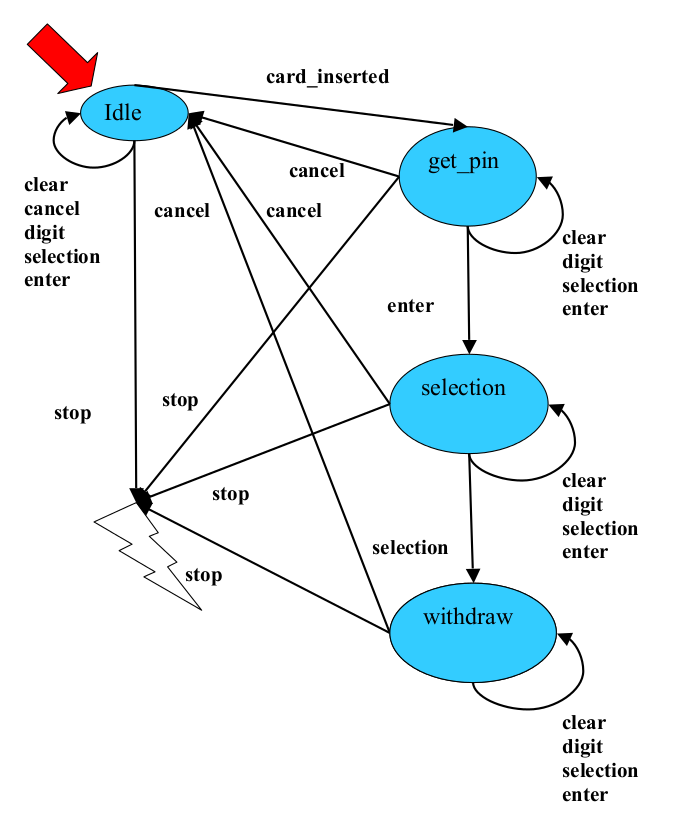
\includegraphics[keepaspectratio=true,height=0.6\paperheight]
{Pictures/ATM_FSM.png}
    \end{center}
     \caption{Example: ATM}
   \label{atm}
\end{figure}


\newpage
\paragraph{Elevator Controller}\ This example contains 7 actor classes.  It 
simulates a system that monitors and schedules a number of elevators.

Figure~\ref{elevator_controller} gives an example elevator controller that 
controls three elevators in a building that has 6 levels.  The three worker 
actors are:
\begin{itemize}
 \item The monitor class that provides a GUI.
 \item The elevator class that models a specific elevator.
 \item The scheduler class that reacts to user inputs.
\end{itemize}

The other 4 actors are supervisors for other components.  The example is 
shipped with QuickCheck properties that checks whether events generated by 
users are correctly handled.



\begin{figure}[p]
     \begin{center}
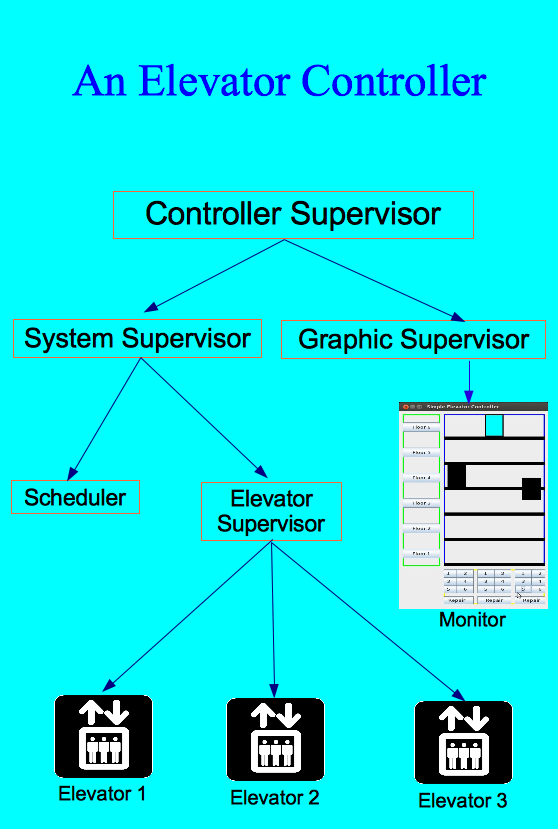
\includegraphics[keepaspectratio=true,height=0.6\paperheight]
{Pictures/ElevatorController.png}
    \end{center}
     \caption{Example:  Elevator Controller}
   \label{elevator_controller}   
\end{figure}

\subsubsection{Examples from the Akka Documentation}

The Akka Documentation \citep{akka_doc} contains some examples that demonstrate 
actor programming and supervision in Akka.  The author has ported the 
following examples to check that applications built using TAkka behave similarly 
to Akka applications.

\paragraph{Ping Pong} This example contains 2 actor classes: {\tt Ping} and 
{\tt Pong}.  The two actors send messages to each other a number of 
times and then terminate.  The example begins with a {\tt ping} message sent 
from a {\tt Ping} actor to a {\tt Pong} actor.  The {\tt Pong} actor replies a 
{\tt pong} message when it receives a {\tt ping} message.  When a {\tt Ping} 
actor receives a {\tt pong} message, it updates its internal message counter.  
If the message counter does not exceed a set number, it sends another {\tt 
Ping} message, otherwise the program terminates.



\paragraph{Dining Philosophers} This example contains 2 actor classes.  It 
models the dining philosophers problem \citep{wiki:philosophers} using 
Finite State Machines (FSMs).   The Dining Philosophers problem is one of the 
classical problems that exhibit 
synchronization issues in concurrent programming.  In the ported version five 
philosophers sit around a table with five chopsticks interleaved.  Each 
philosopher alternately thinks and eats.  Before starting eating, a philosopher 
needs to hold chopsticks on both sides.  At any time, a chopstick can only be 
held by one philosopher.  A philosopher puts down both chopsticks when he 
finishes eating and thinks for a random period.  




\paragraph{Distributed Calculator} This example contains 4 actor classes.  
It demonstrates distributed computation and dynamic behaviour update on the 
receive function of an actor.  The TAkka version of this example is used as a 
case study in Section~\ref{sec_distributed_calculator}.

\paragraph{Fault Tolerance} This example contains 5 actor classes.  It models 
simple key-value data storage.  The data storage maps {\tt String} keys to 
{\tt Long} values.  The data storage throws a {\tt StorageException} when 
users try to save a value between 11 and 14.  The data storage service is 
supervised using the {\tt OneForOne} supervisor strategy.


\subsubsection{Examples from Other Open Source Projects}

The QuviQ examples and the Akka documentation examples are demonstration 
examples for training purposes.  This thesis further ports the following 
examples from open source projects to enlarge the scope of the test.

\paragraph{Barber Shop}  This application has 6 actor classes.  The Akka 
version of this example is implemented by \citet{BarberShop}.  This example
application models the sleeping barber problem \citep{wiki:barber}, which 
involves inter-process communication and synchronization.

\paragraph{EnMAS} This medium size project has 5 actor classes.  The EnMAS 
project, which stands for Environment for Multi-Agent Simulation, is a framework 
for multi-agent and team-based artificial intelligence research \citep{EnMAS}.  
Agents in this framework are actors while specifications are written in DSL 
defined in Scala.


\paragraph{Socko Web Server} The implementation of this application contains 
4 actor classes.  Socko \citep{SOCKO} is a lightweight Scala web server that 
can serve static files and support RESTful APIs.  

\paragraph{Gatling}  This application contains 4 actor classes.  Gatling  
\citep{Gatling} is a stress testing tool for web applications.  It uses actors 
and synchronous I/O methods to improve its efficiency.  The application is 
shipped with a tool that reports test results in graphical charts.

\paragraph{Play Core} The core library of the Play framework only has 1 actor 
class.  The Play framework \citep{play_doc} is part of the TypeSafe stack for 
building web applications.  The Play project is actively maintained by 
developers at TypeSafe Inc. and in the Play community.  Therefore, this project 
only ports its core library which is also updated less frequently.
Because the original Akka Play is an active project on GitHub, a separate repository is 
forked for the TAkka version \citep{takka_play} so that updating non-core components is easier.





\subsection{Evaluation Results}
\label{results}

\subsubsection{Code Size}

This section investigates whether the type discipline enforced by TAkka restricts the 
expressibility of Akka.  Table~\ref{express} lists the examples used for expressiveness checks.  
Medium-seized examples are selected from Quviq \citep{quviq}
and open source Akka projects to ensure that the main requirements for actor 
programming are not unintentionally neglected.  Examples from 
Quviq are re-implemented using both Akka and TAkka.  Examples from 
Akka projects are re-implemented using TAkka.  Following standard practice \citet{Fleming} and \citet{HePa06},  
the author assesses the overall code modification and code 
size by calculating the geometric mean of all examples. The evaluation results 
in Table~\ref{express} show that when porting an Akka program to TAkka, about 
8.5\% lines of code need to be modified including additional type declarations. 
Sometimes, the code size can be smaller because TAkka code does not 
need to handle unexpected messages.  On average, the total program size 
of Akka and TAkka applications are almost the same.  Figure~\ref{fig:expressiveness}
reports the same result in a Scatter chart.



\begin{sidewaystable}[clockwise, p]
\begin{tabular}{| p{4.5 cm} | p{5.6 cm} | c | c |  c | c | c |}
\hline

Source & Example & \specialcell{Akka Code \\ Lines} &
\specialcell{Modified\\ TAkka Lines} & \specialcell{\% of \\Modified Code} &
\specialcell{TAkka Code\\ Lines}
& \specialcell{\% of \\Code Size} \\
\hline
Small   & String Processor & 25 & 11 & 44 & 22 & 88 \\
\cline{2-7}                            
Examples                            & Supervised Calculator &38 & 11 & 29 & 41 & 108 \\ 
\cline{2-7}
                            & Behaviour Upgrade & 38 & 10 & 26 & 39 & 102 \\
\cline{2-7}                            
                            & NQueens & 235 & 6 & 3 & 236 & 100 \\
\cline{2-7}                            
\hline

BenchErl  & bang & 93 & 8 & 8.6 & 94 & 101 \\
\cline{2-7}
Examples                            & big & 93 & 10 & 11 & 100 & 108 \\
\cline{2-7}                            
                            & ehb &201 & 23 & 11 & 216 & 107 \\ 
\cline{2-7}                            
                            & genstress &129 & 12 & 9.3 & 129 & 100 \\ 
\cline{2-7}                            
                            & mbrot & 125 & 8 & 6 & 130 & 104 \\
\cline{2-7}                            
                            & parallel &101 & 9 & 8.9 & 101 & 100 \\ 
\cline{2-7}                            
                            & ran & 98 & 8 & 2.6 & 101 & 103 \\
\cline{2-7}       
                            & serialmsg & 146 & 20 & 14 & 146 & 100 \\
\cline{2-7}       

\hline
QuviQ   & ATM simulator & 1148 & 199 & 17.3 & 1160 & 101 \\
\cline{2-7}
\citep{quviq}    & Elevator Controller & 2850 & 172 & 9.3 & 2878 & 101 \\
\hline
                     & Ping Pong & 67 & 13 & 19.4 & 67 & 100 \\
\cline{2-7}
Akka Documentation   & Dining Philosophers & 189 & 23 & 12.1 & 189 & 100  \\
\cline{2-7}
\citep{akka_doc}     & Distributed Calculator  & 250 & 43 & 17.2 & 250 & 100 \\
\cline{2-7}
                     & Fault Tolerance & 274 & 69 & 25.2 & 274 & 100 \\
\hline

               & Barber Shop \citep{BarberShop}& 754 & 104 & 13.7 & 751 & 99 \\
\cline{2-7}
Other Open Source    & EnMAS \citep{EnMAS} & 1916 & 213 & 11.1 & 1909 & 100 \\
\cline{2-7}
Akka Applications    & Socko Web Server \citep{SOCKO}  & 5024 & 227 & 4.5 & 
5017 & 100 \\
\cline{2-7}
                     & Gatling \citep{Gatling} & 1635 & 111 & 6.8 & 1623 & 99 \\
\cline{2-7}
              & Play Core \citep{play_doc} & 27095 & 15 & 0.05 & 27095 & 100 \\
\hline
geometric mean                   & & 319.5 & 27.4 & 8.6 & 324.4 & 101.5 \\
\hline
\end{tabular}
\caption{Expressiveness Evaluation}
\label{express}
\end{sidewaystable}

\begin{figure}[h]
     \begin{center}
        \subfloat[Code Size: Absolute Lines]{
            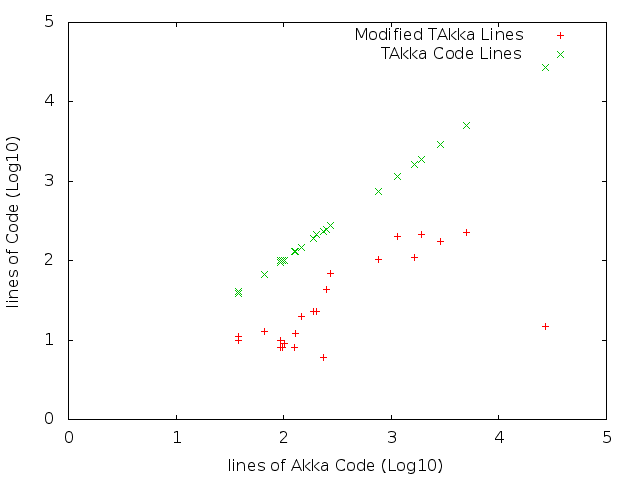
\includegraphics[scale=0.32]{Expressiveness/Expressiveness1.png}
        }
        \subfloat[Code Size: Relative Lines]{
           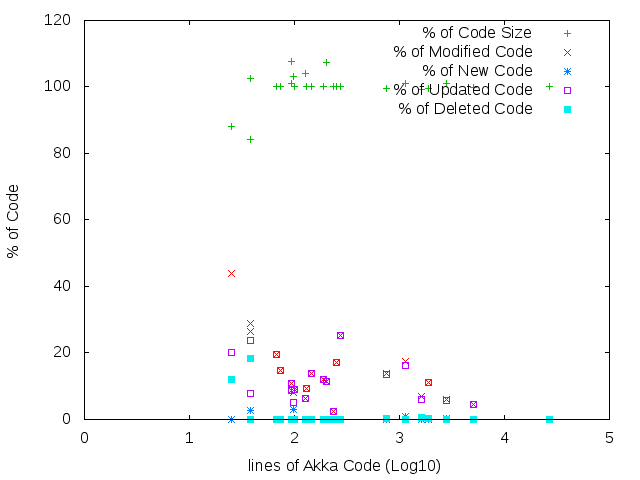
\includegraphics[scale=0.32]{Expressiveness/Expressiveness2.png}
        }
    \end{center}
    \caption{Code Size Evaluation}
   \label{fig:expressiveness}
\end{figure}

\subsubsection{Type Error}

A type error is reported by the compiler when porting the Socko example 
\citep{SOCKO} from its Akka implementation to an equivalent TAkka 
implementation.
Socko is a library for building event-driven web services.  The Socko designer
defines a {\tt SockoEvent} class to be the supertype of all events.  One
subtype of {\tt SockoEvent} is {\tt HttpRequestEvent}, representing events
generated when an HTTP request is received. The designer further implements
subclasses of {\tt Method}, whose {\tt unapply} method intends to pattern
match {\tt SockoEvent} to {\tt HttpRequestEvent}.  The Socko
designer made a type error in the method declaration so that the {\tt unapply}
method pattern matches {\tt SockoEvent} to {\tt SockoEvent}. The type error is
not exposed in test examples because those examples always pass instances 
of {\tt HttpRequestEvent} to the {\tt unapply} method and send the returned
values to an actor that accepts messages of {\tt HttpRequestEvent} type.
Fortunately, the design flaw is exposed when upgrading the Socko implementation 
using TAkka.



\section{Throughput}
\label{throughput}

The Play example \citep{play_doc} and the Socko example \citep{SOCKO} used in 
Section~\ref{expressiveness} are two frameworks for building web services in 
Akka.  A scalable implementation of a web service should be able to have 
a higher maximum throughput when more web servers are added.  Throughput is 
measured by the number of correctly handled requests per unit of time.

The JSON serialization example from the TechEmpower Web Framework benchmarks 
\citep{techempower} checks the maximum throughput achieved during a test.  This 
example is used in this thesis to test how the maximum throughput changes when 
adding more web server applications implemented using Akka Play, TAkka 
Play, Akka Socko, and TAkka Socko.  

For a valid HTTP request sent to path {\tt /json}, e.g. the one given in Figure 
\ref{json_request}, the web service should return a JSON serialization of a new 
object that maps the key message to the value ``Hello, World''.  JSON, which 
stands for JavaScript Object Notation, is a language independent format for 
data exchange between applications \citep{json}.  Figure~\ref{json_response} 
gives an example of an expected HTTP response.  The body of the example 
response, line 7, is the expected JSON message.


\lstset{language=html}

\begin{figure}[!h]
\begin{center}
  \subfloat[An Example HTTP Request]{%
  \label{json_request}
  \lstinputlisting{code/json_request}%
}
\hfill
  \subfloat[An Example HTTP Response]{%
  \label{json_response}
  \lstinputlisting{code/json_response}%
}
  \caption{Example: JSON serialization Benchmark}
\end{center}    
  \label{json_example}
\end{figure}
\lstset{language=scala}


All four versions of the web service were deployed to servers on Amazon 
Elastic Compute Cloud (EC2) \citep{ec2}.  The example was tested with up to 16 
EC2 micro instances (t1.micro), each of which had 0.615 GB Memory.   The author 
expected that web servers built using an Akka-based library and a TAkka-based 
library would have similar throughput.


To avoid pitfalls mentioned in \citep{pitfall}, a FreeBench \citep{freebench} 
tool was designed and implemented for benchmarking throughputs of HTTP 
servers.  One feature of the FreeBench tool is that it can benchmark web 
servers deployed at multiple addresses.  In the JSON serialization benchmark, 
the maximum throughput achieved when using the Elastic Load Balancing (ELB) 
service \citep{elb} did not obviously increase when more servers were added. 
In contrast, when all deployed EC2 servers were benchmarked, the 
total throughput increased slightly. One possible explanation for the above 
observation is that the benchmark is bounded by the throughput of ELB,
which runs on a micro EC2 instance.  Another 
feature of the FreeBench tool is that it can be configured to carry out a 
number of benchmarks in parallel and repeat the parallel benchmark a 
certain number of times.  The benchmark results of all tests are sent to a data 
store which reports a customised statistical summary.

The parameters set in this example were the number of EC2 instances used.  For 
each of the four types of server, the example was tested with up to 16 
EC2 instances.  For each number of EC2 instances, 10 rounds of benchmarking 
were executed. In each round, 20 sub-benchmarks were carried out in parallel to 
maximise the utility of broadband.  For each sub-benchmark, 10,000 requests were
sent.  The upload and download speed were manually monitored to confirm that 
the network speed was stable for most of the time during the test with the 
above configurations.

Figure~\ref{fig:throughput} summarises the results of the JSON serialization 
benchmark.  It shows the average and the standard deviation of the throughput 
in each test.  The result shows that web servers built using an Akka-based 
library and a TAkka-based library have similar throughput.  The micro example
used in this test does not show a good throughput scalability in both Akka
and TAkka versions.  It will be more interesting if we can benchmark on a real Akka web service
whose throughput is linear to the number of available servers.






\begin{figure}[h]
     \begin{center}
        \subfloat[]{
            \label{fig:play_throughput}
            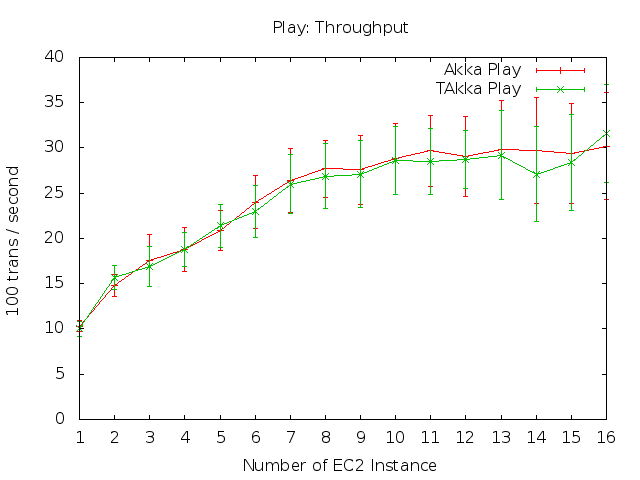
\includegraphics[scale=0.32]{Play_throughput.png}
        }
        \subfloat[]{
           \label{fig:socko_throughput}
           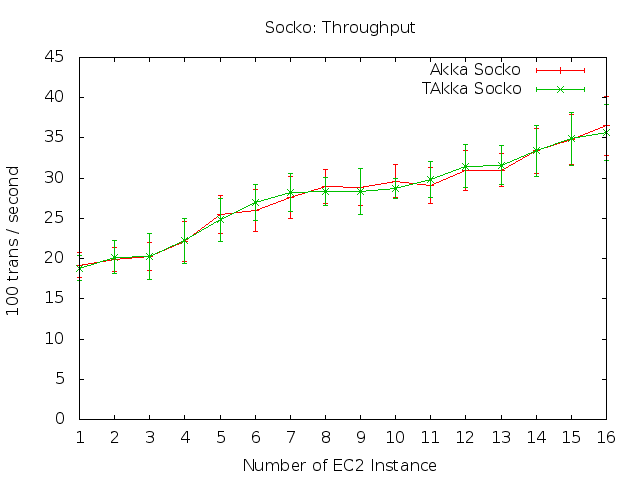
\includegraphics[scale=0.32]{Socko_throughput.png}
        }
    \end{center}
     \caption{Throughput Benchmarks}
   \label{fig:throughput}
\end{figure}

\newpage
\section{Efficiency and Scalability}
\label{efficiency}




The TAkka library is built on top of Akka so that code for shared features 
can be re-used.  The main sources of overheads in the TAkka implementation
are:

\begin{enumerate}[i)]
  \item the cost of adding an additional operational layer on top of Akka 
code,
  \item the cost of constructing type descriptors,
  \item the cost of transmitting type descriptors in distributed settings, and
  \item the cost of dynamic type checking when registering new typed names.
\end{enumerate}

The upper bounds of costs i) and ii) were assessed by a micro 
benchmark which assessed the time for initializing {\it n} instances of {\tt 
StringCounter} defined in Figure~\ref{fig:akka_string_counter} and Figure 
\ref{takka_string_counter}. When {\it n} ranges from $10^4$ to $10^5$, as 
shown in Figure~\ref{cost_of_type}, the TAkka implementation runs roughly 
half as fast as the Akka implementation.  


\vspace{15pt}
\begin{figure}[h]
\begin{center}
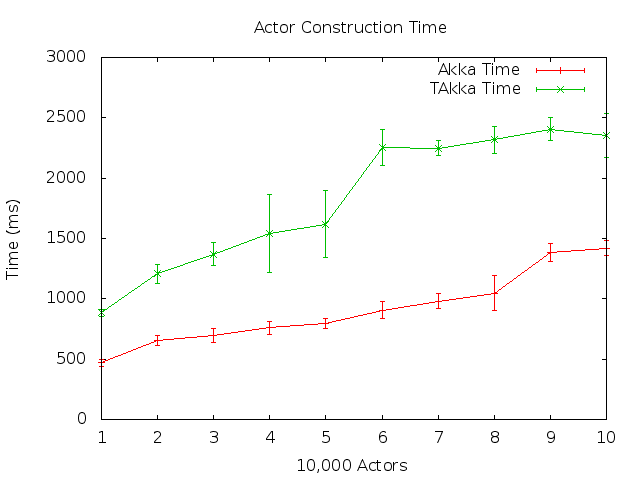
\includegraphics[scale=0.6]{efficiency/Actor_Construction.png}
\caption{Cost of Actor Construction}
\label{cost_of_type}
\end{center}
\end{figure}

\newpage

The cost of transmitting a type descriptor should be close to the cost of 
transmitting the string representation of its fully qualified type name.  The 
relative overhead of the latter cost depends on the cost of computations 
spent on application logic.

TAkka applications that have a relatively heavy computation cost should have 
similar runtime efficiency and scalability compared with equivalent Akka 
applications because static type checking happens at compile time and dynamic 
type checking is usually not the main cost of applications that involve other 
meaningful computations.  To confirm the above expectation, the speed-up of 
multi-node TAkka applications was further investigated by porting 
appropriate micro benchmark examples from the BenchErl benchmarks in the 
RELEASE project \citep{RELEASE, aronis2012scalability}. 


\subsection{BenchErl Overview}
\label{bencherl_overview}

BenchErl \citep{RELEASE, aronis2012scalability} is a scalability benchmark suite 
for applications written in Erlang.  It includes a set of micro benchmark 
applications that assess how an application changes its performance when 
additional resources (e.g. CPU cores, schedulers, etc.) are added.  This thesis 
uses BenchErl examples, which do not involve OTP ad-hoc libraries, to 
investigate how the performance of an application changes when more distributed 
nodes are added.

All BenchErl examples are implemented in a similar structure.  Each BenchErl 
benchmark spawns one master process and a configurable number of child 
processes.  Child processes are evenly distributed across available 
potentially distributed nodes.  The master process asks each child process to 
perform a task and send the result back to the master process.  Finally, when 
results are collected from all child processes, the master process assembles 
them and reports the overall elapsed time for the benchmark.

BenchErl examples have similar structure to the MapReduce model 
\citep{dean2008mapreduce}, which matches many real world tasks.  More 
importantly, those programs are automatically parallelized when executed on 
a cluster of machines.  This pattern allows benchmark users to focus on the 
effects of changes in computational resources rather than specific 
parallelization and scheduling strategies of each example.






\newpage

\subsection{Benchmark Examples}

\subsubsection{Ported BenchErl Examples}
\label{ported_examples}

The following BenchErl examples were ported for comparing the efficiency 
and scalability of applications built using TAkka and Akka:

\paragraph{bang}  This benchmark tests many-to-one message passing.  The child 
processes spawned in this example are {\it sender} actors which send the 
master process a fixed number of dummy messages.  The master process 
initializes a counter, set to the product of the number of processes and the 
number of messages expected from each child.  When a dummy message is received, 
the master counts down the number of remaining expected messages.  The 
benchmark example completes when all expected messages are received.  

Parameters set in this example are the number of available nodes, the 
number of child processes to spawn, and the number of messages sent by each 
child process.  Instead of carrying out computations, the main task of this 
benchmark is sending messages from child processes to the master process.  
Therefore, the benchmark is likely to be bounded by throughput of the master node.


\paragraph{big}  This benchmark tests many-to-many message passing.  A child 
process in this example sends a {\tt Ping} message to each of the other child 
processes.  Meanwhile, each child replies with a {\tt Pong} message when it 
receives a {\tt Ping} message.  Therefore, if $n$ child processes are spawned, 
each child is expected to send $n-1$ messages and receive $n-1$ messages from 
others.  When a child completes the task, it sends a {\tt BigDone} message to 
the master actor.  The benchmark example completes when the master actor 
receives {\tt BigDone} messages from all of its children.  

Parameters set in this example are the number of available nodes and the number 
of child processes to spawn.  The main task of 
this benchmark is sending messages rather than computations.  For each child 
process, the number of messages it sends and receives is linear to the total 
number of child processes.  Similarly to the {\tt bang} example, the benchmark 
is likely to be bounded by throughput of the master node.


\paragraph{ehb} This benchmark re-implements the hackbench example 
\citep{hackbench} originally used for stress testing Linux schedulers.  
Each child process in this benchmark is a group of message senders and 
receivers.  Each sender sends each receiver a dummy message and waits for an 
acknowledge message.  Each sender repeats the process a number of times.  
When a sender has received all expected replies, it reports to the child actor 
that it has completed its task.  When all senders in the group have completed 
their tasks, the child process sends a complete message to the master process.  
The benchmark completes when all child processes have finished their tasks. 

Parameters set in this example are the number of available nodes, the number 
of groups, group size, and the number of loops.  Let $n$ be the number of 
groups in this benchmark, and $m$ be the number of senders and receivers in 
each group.  The master process then expects $n$ messages while a total of 
$2m^2$ messages are sent in each group.  Therefore, the main task of this 
benchmark is sending messages inside each group.  When the number of
available nodes to share the task of child processes is increased, this 
benchmark is expected to have shorter runtime.


\paragraph{genstress}  This benchmark is similar to the bang test.  It spawns an
echo server and a number of clients.  Each client sends some dummy messages to
the server and waits for its response.  When a client receives the response, 
it sends an acknowledge message to the master process.  The benchmark completes 
when results from all child processes are received.  There are two versions 
in Erlang, one using the OTP {\it gen\_server} behaviour, the other 
implementing a simple server-client structure manually.  This 
benchmark ports the version not using {\it gen\_server}.  

Parameters set in this example are the number of available nodes, the number 
of child client processes to spawn, and the number of messages sent by each 
child process. The main task of this benchmark is sending messages from child 
processes to the master process. Therefore, the benchmark is likely to be bounded by throughput of the master node.

\paragraph{mbrot} This benchmark models pixels in a 2-D image of a specific 
resolution.  For each pixel at a given coordinate, the benchmark determines 
whether it belongs to the Mandelbrot set \citep{wiki:mandelbrot} or not. The 
determination process usually requires a large number of iterations.  In this 
benchmark, child processes share roughly the same number of points.  The 
benchmark completes when all child processes have finished their tasks.

Parameters set in this example are the number of available nodes, the number 
of child processes to spawn, and the dimensions of the image.  Keeping the 
dimensions of the image to be a medium fixed size, with more available nodes to 
share the computation task, this benchmark is expected to have shorter runtime.




\paragraph{parallel}  This benchmark spawns a number of child processes.  Each 
child process creates a list of $N$ timestamps and checks that elements of the 
list are strictly increased, as promised by the implementation of the {\it now} 
function.  After completing the task, the child process sends the result list 
to the master process.  The benchmark completes when results from all child 
processes are received.

Parameters set in this example are the number of available nodes, the number of 
child processes, and the number of timestamps each child creates. Compared to 
the cost of creating timestamps and comparing data locally, the cost of sending 
distributed messages is usually much higher.  Therefore, the runtime of this 
benchmark is likely to be bounded by the task of sending results to the 
master process.




\paragraph{ran}  This benchmark spawns a number of processes.  Each child 
process generates a list of 100,000 random integers, sorts the list using 
quicksort, and sends the first half of the result list to the master process.  
The benchmark completes when results from all child processes are received.

Parameters set in this example are the number of available nodes and the 
number of child processes to spawn. For each child process, the cost of 
generating integers is linear to the number of integers, and the cost of 
sorting is linear logarithmically to the number of integers.  If the number of 
generated integers in each child process is increased so that the cost of 
communicating with the master process can be neglected, this benchmark is a 
good example for a scalability test.  Unfortunately, the space cost of this 
example also increases when the number of generated integers is increased.  In 
the TAkka and Akka benchmarks, the cost of garbage collection by JVM cannot be 
neglected when the number of generated integers is set to a higher number.


\paragraph{serialmsg} This benchmark tests message forwarding through a
dispatcher.  This benchmark spawns one proxying process and a number of 
pairs of message generators and message receivers.  Each message 
generator creates a random short string message and asks the proxying process 
to forward the message to a specific receiver.  A receiver sends the master 
process a message when it receives the message.  The benchmark completes when 
the master process receives messages from all receivers.

The parameters set in this example are the number of available nodes, the 
number of pairs of senders and receivers,  the number of messages and the 
message length.  Clearly, this benchmark is bounded by the throughput
of the proxying process when the speed of 
generating messages exceeds the speed of forwarding messages.


\subsubsection{BenchErl Examples that are Not Ported}

The following BenchErl examples are not ported for reasons given in respective 
paragraphs.

\paragraph{ets\_test} ETS table is an Erlang build-in module for concurrently 
saving and fetching shared global terms  \citep{ErlangManual}.  This benchmark 
creates an ETS table.  Child processes in this benchmark perform insert and 
lookup operations to the created ETS table a number of times.  This example 
is not ported because it uses ETS table, a feature that is specific to the 
Erlang OTP platform.

\paragraph{pcmark} Similarly to the {\it ets\_test} example, this benchmark 
also tests ETS operations.  In this benchmark, five ETS tables are created. 
Each created table is filled with some values before the benchmark begins.  The 
benchmark spawns a certain number of child processes that read the content of 
those tables.  This example is not ported either because it uses the ETS table.


\paragraph{timer\_wheel} Similarly to the {\it big} example, this benchmark 
spawns a number of child processes that exchange ping and pong messages.  
Differently to the {\it big} example, processes in this example can be 
configured to await reply messages only for a specified timeout.  In cases where 
no timeout is set, or it is set to a short period, this example is the same 
as the {\it big} example.  If a timeout is set to a long period, the 
runtime of this example is bounded by the timeout.  For the above reason, this 
example is not ported.



\newpage


\subsection{Benchmark Methodology}
\subsubsection{Testing Environment}

The benchmarks were run on a 32 node Beowulf cluster at Heriot-Watt 
University.  The 32 Beowulf cluster nodes each comprise eight Intel 5506 cores 
running at 2.13GHz. All machines run under Linux CentOS 5.5. The Beowulf 
nodes are connected with Baystack 5510-48T switches with 48 10/100/1000 ports.

\subsubsection{Determining Parameters}
\label{bench_parameters}

The main interest of the efficiency and scalability test is to check whether 
applications built using Akka and TAkka have similar efficiency and 
scalability.  Meanwhile, our secondary interest is to know how 
the required run-time of a BenchErl example changes when more 
machines are employed.  Ideally, for each comparison on the efficiency of 
an Akka application and its equivalent TAkka application, the only variable 
should be the number of employed nodes.  Nevertheless, the BenchErl examples 
listed in Section~\ref{ported_examples} have more parameters to be configured.  
Experiments for our main interests can be carried out with any 
parameters, however; for consideration of our secondary interest, 
parameters for each example were selected according to the following three 
criteria:

First, except for the RAN example, the runtime of each experiment was 
constrained to be 40 seconds.  The decision was made so that the time to 
measure each example was acceptable.  As will be explained in the next 
section, each example was tested for a total of 90 rounds of experiments.  
Another reason for this decision was that the experiment should be able to 
complete in a reasonably short time when running on a single machine.  During 
the experiment, the author observed some configurations such that an example 
had a bad performance when run on a single machine but sped up by a factor 
bigger than the total number of available nodes when run with more nodes.  
These experiments give interesting results that proved the importance of 
distributed programming; however, it is desired that the number of nodes be the 
only independent variable throughout all experiments.  Therefore, the 
benchmarks preferred configurations that neglected the impact of other factors 
such as garbage collection.

Second, the benchmarks preferred configurations that had more workload for each 
child process. In a number of tests to determine parameters, the author 
observed employing more machines only had runtime benefit for those 
BenchErl examples whose runtime is bounded by the computational tasks rather 
than the throughput of the only master process.

Third, the benchmarks preferred configurations that had more child processes 
but did not violate the above two principles.  The benchmark was run on 
a maximum of 32 Beowulf machines.  Although each machine has 8 CPU cores, the 
number of CPU cores used to execute Akka and TAkka applications is not 
guaranteed.  For each example, it is started with a small number of child 
processes.  If the child process could have a higher workload by setting other 
parameters, other parameters were changed until the configuration violated the 
first criterion.  If the number of child processes and the number of available 
nodes were the only two parameters, or the workload of each child process did 
not change significantly with other possible configurations, the number of child 
processes was increased gently until the example took a long time to be 
completed on a single machine.

Based on the results of trial experiments, the parameters used in each 
example were as follows:

\paragraph{bang} 

\begin{itemize}
  \item number of child processes: 512
  \item number of messages sent by each child process: 2000
\end{itemize}

\paragraph{big} 
\begin{itemize}
  \item number of child processes: 1024
\end{itemize}

\paragraph{ehb}  

\begin{itemize}
  \item number of groups: 128
  \item group size: 10
  \item number of loops: 3
\end{itemize}

\paragraph{genstress}  

\begin{itemize}
  \item number of child processes: 64
  \item number of messages sent by each child process: 300
\end{itemize}


\paragraph{mbrot} 

\begin{itemize}
  \item number of child processes: 256
  \item dimensions of the image: 6000x6000
\end{itemize}


\paragraph{parallel}

\begin{itemize}
  \item number of child processes: 256
  \item number of timestamps each child to create: 6000
\end{itemize}



\paragraph{ran} 
\begin{itemize}
  \item number of child processes: 6000
  \item list size: 100000
\end{itemize}


\paragraph{serialmsg}

\begin{itemize}
  \item number of pairs of senders and receiver: 256
  \item number of messages: 100
  \item message size: 200 characters
\end{itemize}

\subsubsection{Measurement Methodology}

After determining the benchmark parameters for each example, the runtime of 
each program was measured as follows.  First, each benchmark contains nine 
tests that use different numbers of Beowulf nodes.  The number of nodes 
used in the benchmarks were 1, 4, 8, 12, 16, 20 , 24, 28, and 32.  Similarly 
to the Benchmark Harness process in \citep{blackburn2006dacapo}, test results 
was recorded after a number of dry-runs to warm-up the runtime environment.  
After the warm-up period, the test was run 10 times.  The 
run time was recorded for later analysis.  Following guidance given by 
\citet{Fleming} and \citet{HePa06}, the efficiency of each example 
using a specific number of nodes is reported by giving the average and standard 
deviation of the 10 runs.  The speed-up of a benchmark example using $n$ nodes 
is measured as the proportion of the average time with one node and the average 
time with $n$ nodes.  After each test, the runtime environment was cleaned up  
before changing the number of nodes or switching to another benchmark example.

\subsection{Evaluation Results}

The records of the BenchErl benchmarks are summarised in Figure 
\ref{runtime_efficiency}.  The efficiency results include both the average 
runtime and the standard deviation.  The scalability results are computed based 
on the average runtime.  The author observes the following though benchmarking:

\paragraph{Observation 1} In all examples, TAkka and Akka implementations had 
almost identical run-times and hence have similar scalability.  In Figure 
\ref{runtime_efficiency}, the runtime of Akka benchmarks and TAkka benchmarks 
often overlay each other.  For benchmarks that do not overlay, the 
difference is less than 10\% on average.  The scalability of Akka applications 
and the scalability of their TAkka equivalents appear slightly different 
because their differences are amplified by their runtime differences when 
running on a single node.

\paragraph{Observation 2} Some benchmarks scale well when more nodes are added. 
 Examples of this observation are the {\tt EHB} example and the {\tt MBrot}. 

\paragraph{Observation 3} Some benchmarks only scale well when a small number 
of nodes are added.  These examples do not scale when the number of nodes are 
greater than a certain number.  Examples of this observation are the {\tt Bang} 
example, the {\tt Big} example, and the {\tt Ran} example.  The speed-up of 
those examples does not further increase when the number of nodes is more than 
four or eight.  

\paragraph{Observation 4} Some benchmarks do not scale.  Examples of this 
observation are the {\tt GenStress} example and the {\tt Parallel} 
example, and the {\tt SerialMsg} example.




\begin{figure}[p]
     \begin{center}
        \subfloat[Bang Time]{
            \label{fig:1a}
            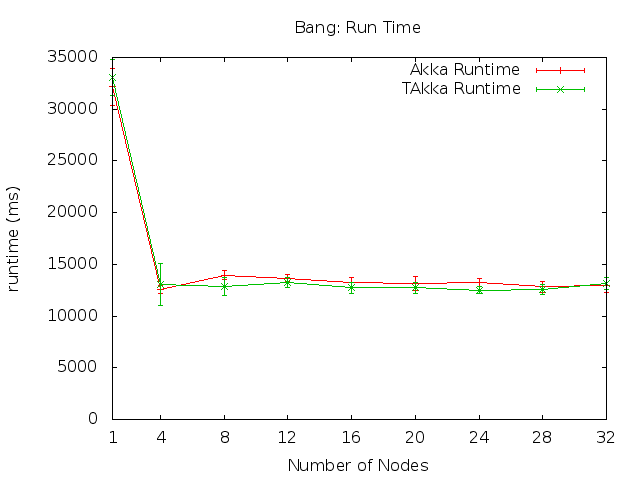
\includegraphics[scale=0.31]{efficiency/Bang_time.png}
        }
        \subfloat[Bang Scalability]{
           \label{fig:1b}
           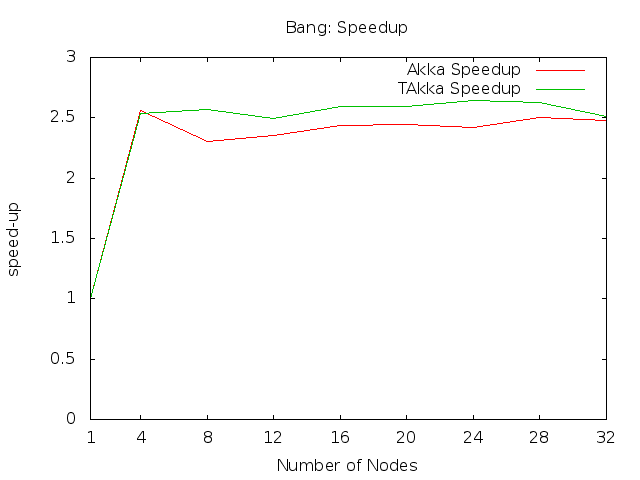
\includegraphics[scale=0.31]{efficiency/Bang_speedup.png}
        }\\
        \subfloat[Big Time]{
            \label{fig:1c}
            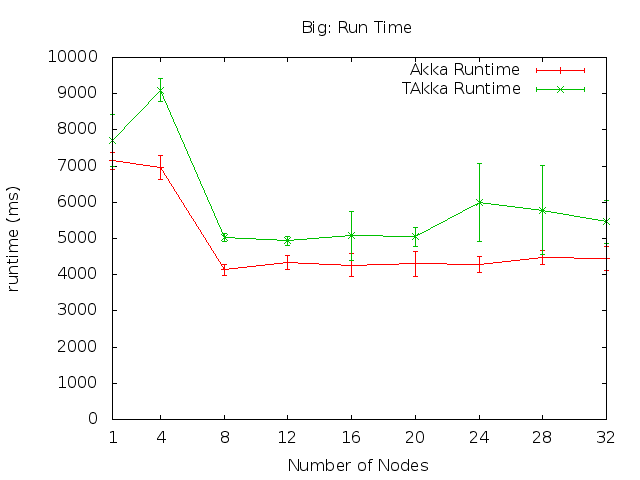
\includegraphics[scale=0.31]{efficiency/Big_time.png}
        }
        \subfloat[Big Scalability]{
           \label{fig:1d}
           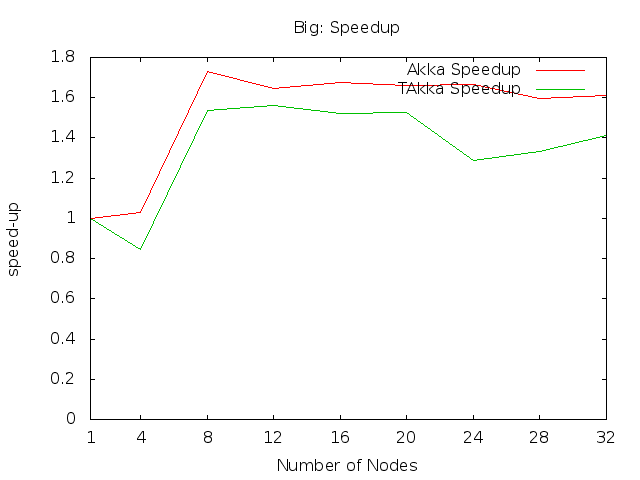
\includegraphics[scale=0.31]{efficiency/Big_speedup.png}
        }\\
        \subfloat[EHB Time]{
            \label{fig:1e}
            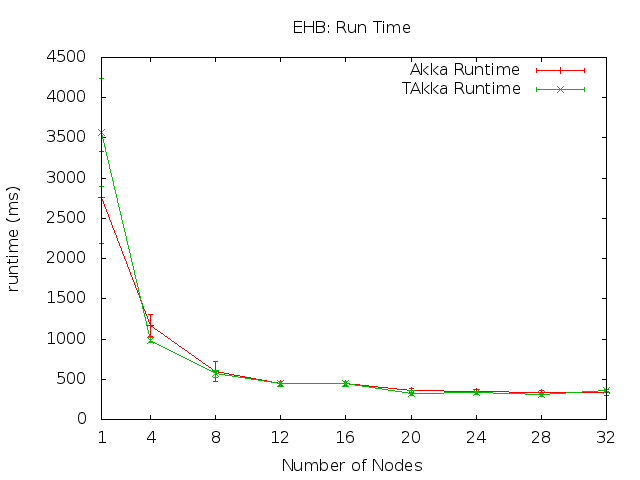
\includegraphics[scale=0.31]{efficiency/EHB_time.png}
        }
        \subfloat[EHB Scalability]{
           \label{fig:1f}
           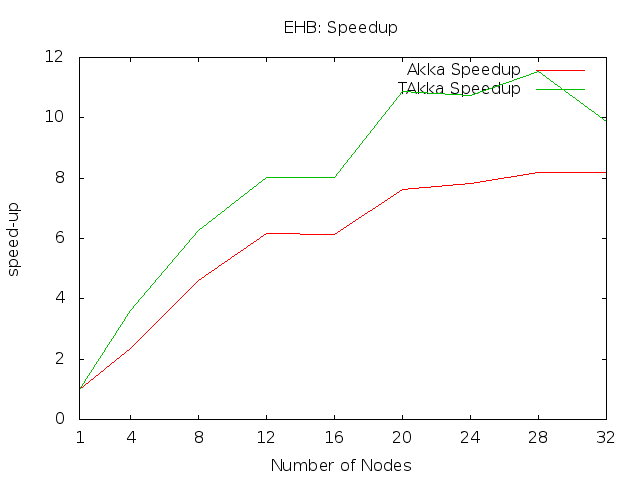
\includegraphics[scale=0.31]{efficiency/EHB_speedup.png}
        }\\
    \end{center}
    \caption{Runtime and Efficiency Benchmarks}
%   \label{runtime_efficiency}
\end{figure}
\begin{figure}[p]
    \ContinuedFloat
     \begin{center}
        \subfloat[GenStress Time]{
           \label{fig:1g}        
            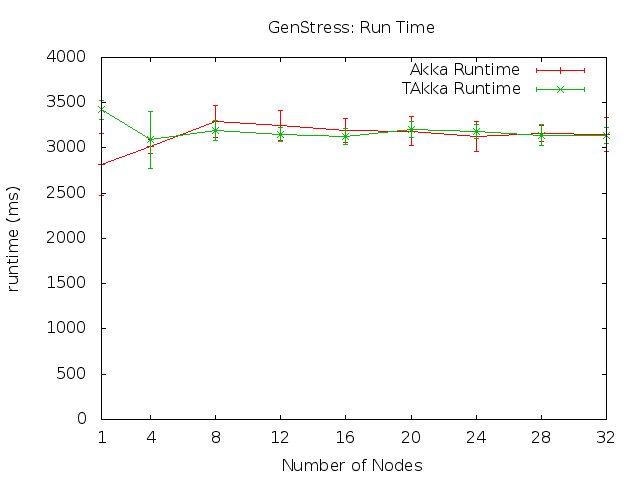
\includegraphics[scale=0.31]{efficiency/GenStress_time.png}
        }
        \subfloat[GenStress Scalability]{
           \label{fig:1h}
           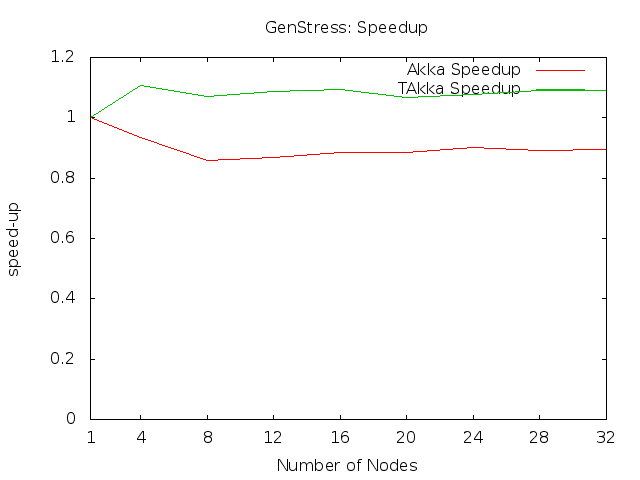
\includegraphics[scale=0.31]{efficiency/GenStress_speedup.png}
        }\\
        \subfloat[MBrot Time]{
            \label{fig:1i}
            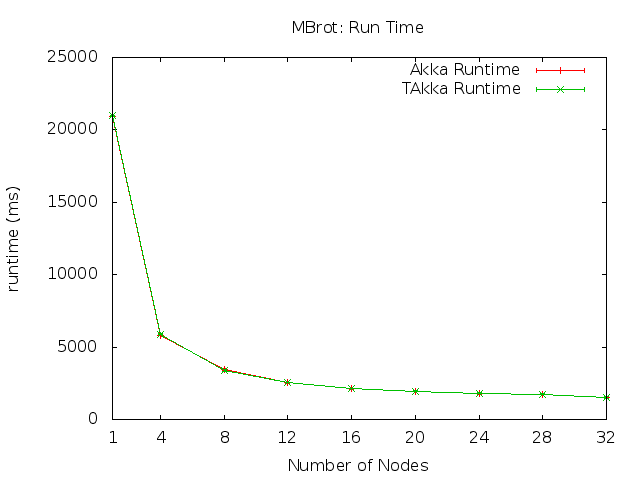
\includegraphics[scale=0.31]{efficiency/MBrot_time.png}
        }
        \subfloat[MBrot Scalability]{
           \label{fig:1j}
           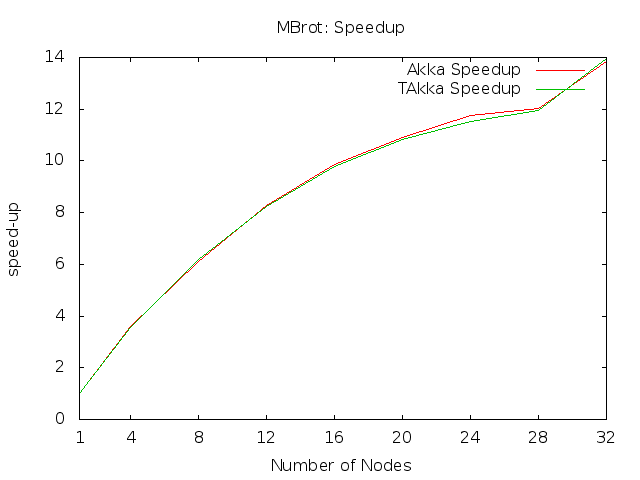
\includegraphics[scale=0.31]{efficiency/MBrot_speedup.png}
        }\\
        \subfloat[Parallel Time]{
            \label{fig:1k}
            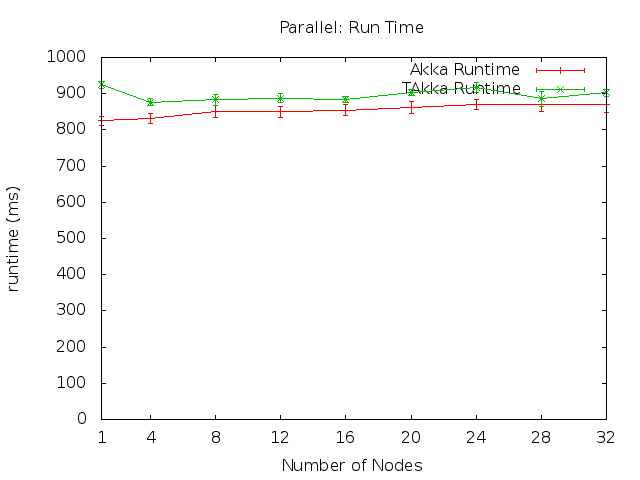
\includegraphics[scale=0.31]{efficiency/Parallel_time.png}
        }
        \subfloat[Parallel Scalability]{
           \label{fig:1l}
           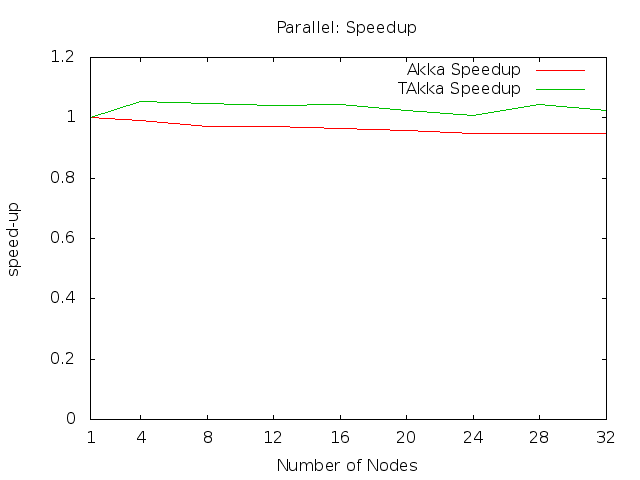
\includegraphics[scale=0.31]{efficiency/Parallel_speedup.png}
        }\\
    \end{center}
    \caption{Runtime and Efficiency Benchmarks}
%   \label{runtime_efficiency}
\end{figure}
\begin{figure}[p]
    \ContinuedFloat
     \begin{center}
        \subfloat[RAN Time]{
            \label{fig:1m}
            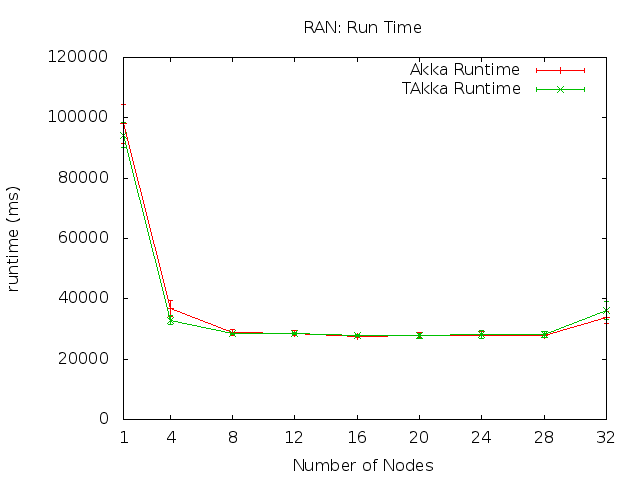
\includegraphics[scale=0.31]{efficiency/RAN_time.png}
        }
        \subfloat[RAN Scalability]{
           \label{fig:1n}
           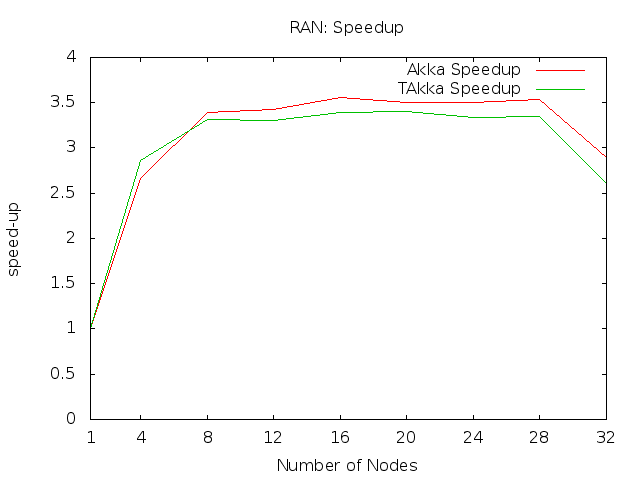
\includegraphics[scale=0.31]{efficiency/RAN_speedup.png}
        }\\
        \subfloat[SerialMsg Time]{
            \label{fig:1o}
            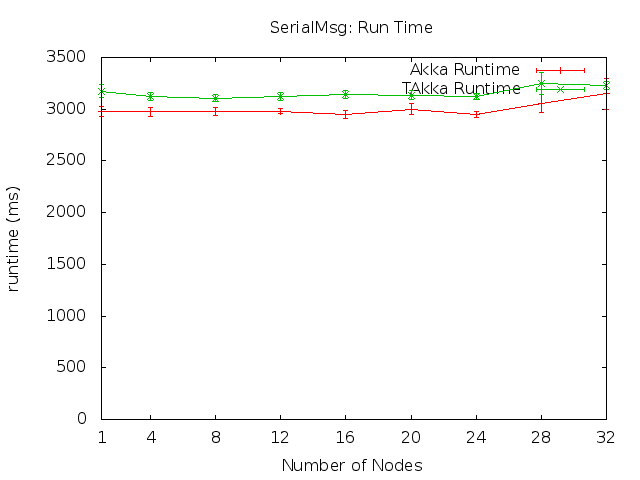
\includegraphics[scale=0.31]{efficiency/SerialMsg_time.png}
        }
        \subfloat[Serial Scalability]{
           \label{fig:1p}
           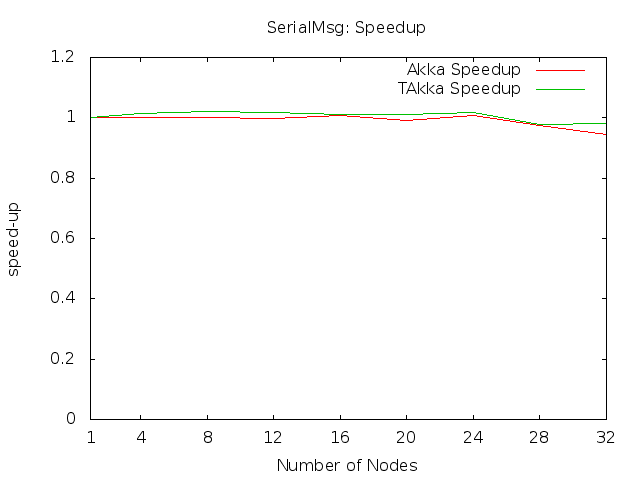
\includegraphics[scale=0.31]{efficiency/SerialMsg_speedup.png}
        }\\
    \end{center}
    \caption{Runtime and Efficiency Benchmarks}
   \label{runtime_efficiency}
\end{figure}


\newpage

\subsection{Additional Benchmarks}
\label{bench_fib}

\subsubsection{Fibonacci Numbers}

Results given in the last section show that the scalability of BenchErl 
examples varies.  Because BenchErl examples have similar structure and those 
examples are run on the same environment, the difference in their scalability 
may lie in differences in their computational tasks.  It is expected 
that the required runtime of a BenchErl example would depend on the time needed 
for completing the computation task and the time for assembling results.  
Because the master process is the only one that assembles the results, a 
BenchErl benchmark is $not$ likely to give a good scalability if most of its 
time is spent on collecting and processing the results of child processes.

To confirm that the scalability of a BenchErl benchmark depends on the ratio 
of the time spent on completing parallelized computational tasks and that spent 
on assembling results, a similar benchmark example was added, where each child 
process computes the {\it same} Fibonacci number {\it sequentially} using the following equation.

\begin{equation}
 f(n) = \begin{cases} 
            1,             & \mbox{if } n = 0 \ { or }\  n = 1  \\ 
            f(n-1)+f(n-2), & \mbox{if } n >=2
         \end{cases}
\end{equation}

The above basic way of computing a Fibonacci number was chosen because it has 
an exponential complexity to the input $n$, and hence the time to compute 
$f(n)$ changes dramatically when $n$ changes.

The parameters set in this example are the number of available nodes, the 
number of child processes, and the value of $n$ in $f(n)$.  The author expected 
that, when setting the number of child processes to a number higher 
than the number of available nodes, a benchmark with a higher $n$ would give 
better scalability than those with a lower $n$.  The above expectation
is confirmed by the benchmark result reported in Figure~\ref{fib_efficiency}.

\begin{figure}[p]
     \begin{center}
        \subfloat[Fib20 Time]{
            \label{fig:1q}
            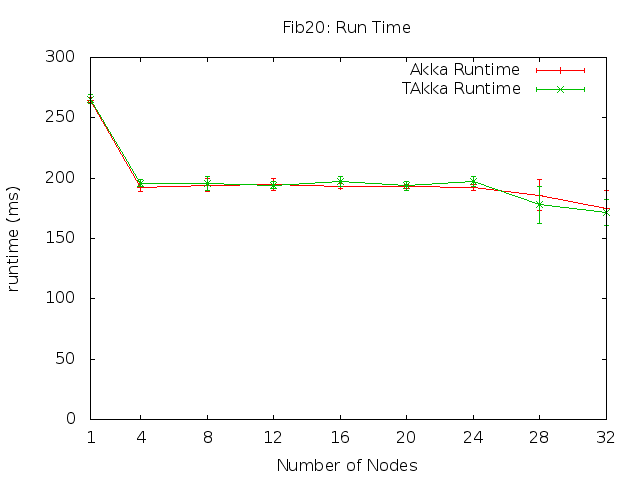
\includegraphics[scale=0.31]{efficiency/Fib20_time.png}
        }
        \subfloat[Fib20 Scalability]{
           \label{fig:1r}
           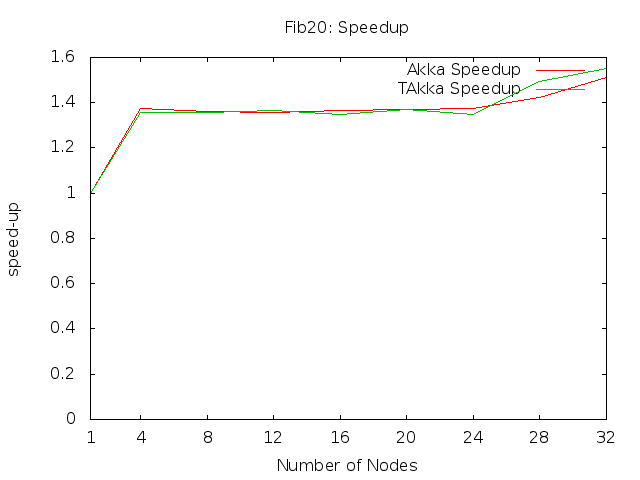
\includegraphics[scale=0.31]{efficiency/Fib20_speedup.png}
        }\\
        \subfloat[Fib30 Time]{
            \label{fig:1s}
            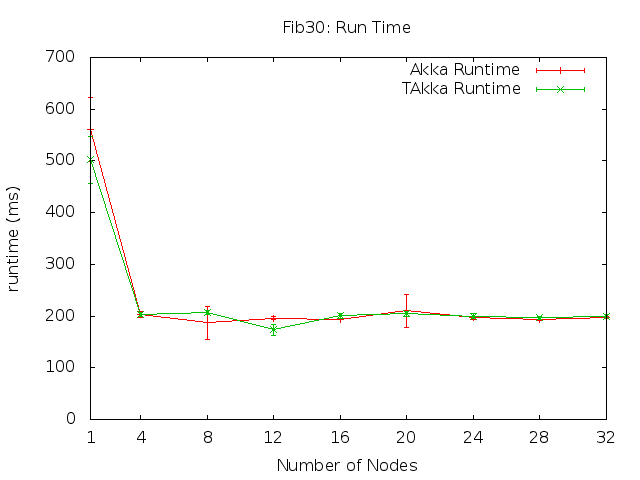
\includegraphics[scale=0.31]{efficiency/Fib30_time.png}
        }
        \subfloat[Fib30 Scalability]{
           \label{fig:1t}
           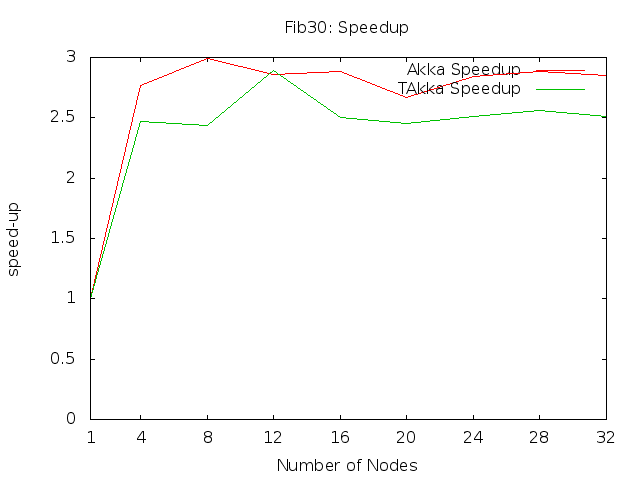
\includegraphics[scale=0.31]{efficiency/Fib30_speedup.png}
        }\\
        \subfloat[Fib40 Time]{
            \label{fig:1u}
            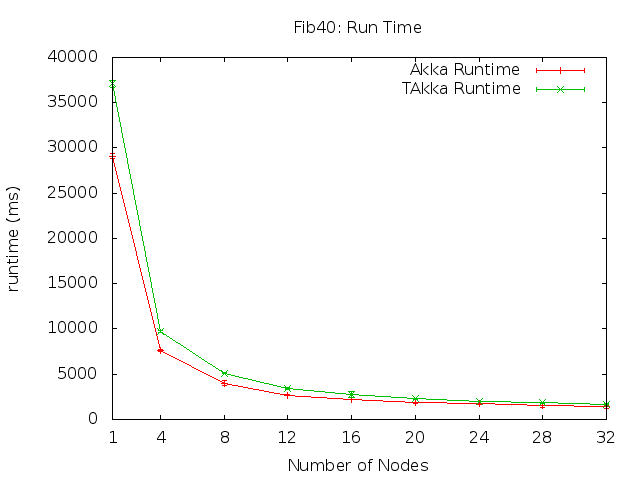
\includegraphics[scale=0.31]{efficiency/Fib40_time.png}
        }
        \subfloat[Fib40 Scalability]{
           \label{fig:1v}
           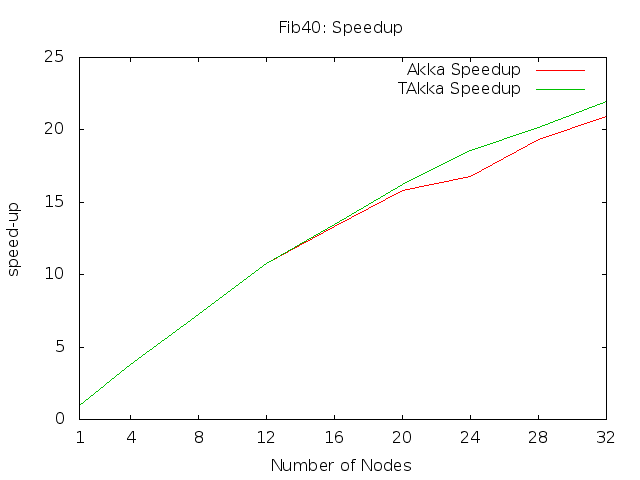
\includegraphics[scale=0.31]{efficiency/Fib40_speedup.png}
        }\\
    \end{center}
    \caption{Benchmark:Parallel Fibonacci Numbers}
   \label{fib_efficiency}
\end{figure}

\subsubsection{MBrot with different image sizes}

\begin{figure}[p]
     \begin{center}
        \subfloat[MBrot10 Time]{
            \label{fig:1q}
            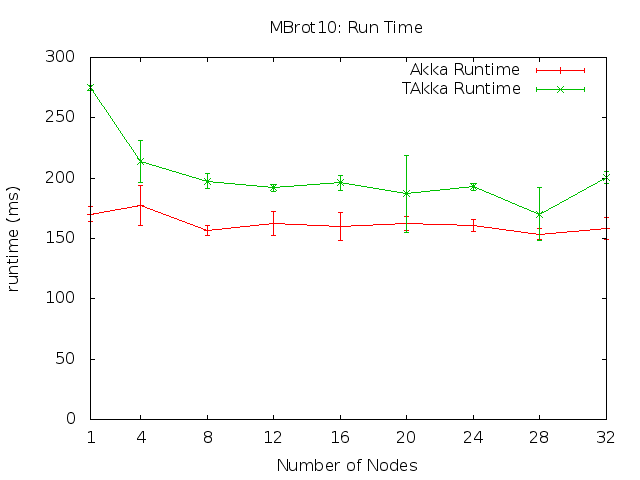
\includegraphics[scale=0.31]{efficiency/MBrot10_time.png}
        }
        \subfloat[MBrot10 Scalability]{
           \label{fig:1r}
           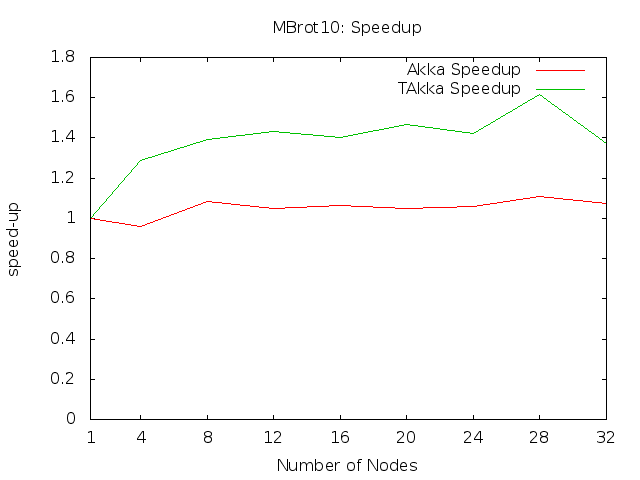
\includegraphics[scale=0.31]{efficiency/MBrot10_speedup.png}
        }\\
        \subfloat[MBrot1000 Time]{
            \label{fig:1s}
            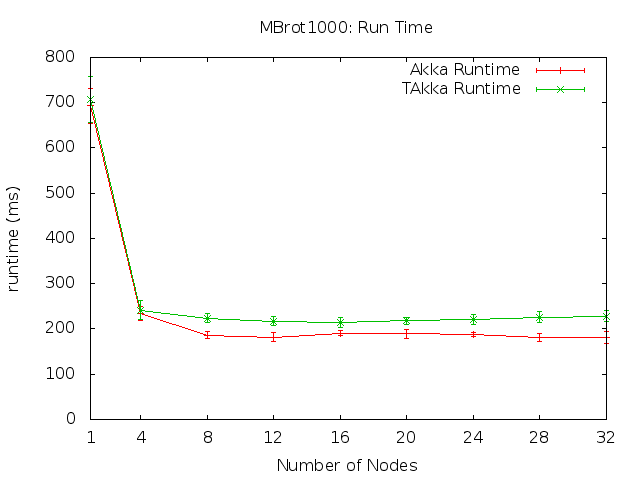
\includegraphics[scale=0.31]{efficiency/MBrot1000_time.png}
        }
        \subfloat[MBrot1000 Scalability]{
           \label{fig:1t}
           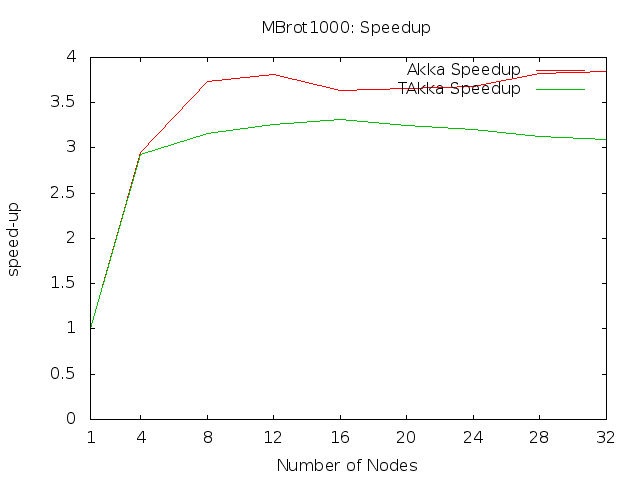
\includegraphics[scale=0.31]{efficiency/MBrot1000_speedup.png}
        }\\
        \subfloat[MBrot6000 Time]{
            \label{fig:1u}
            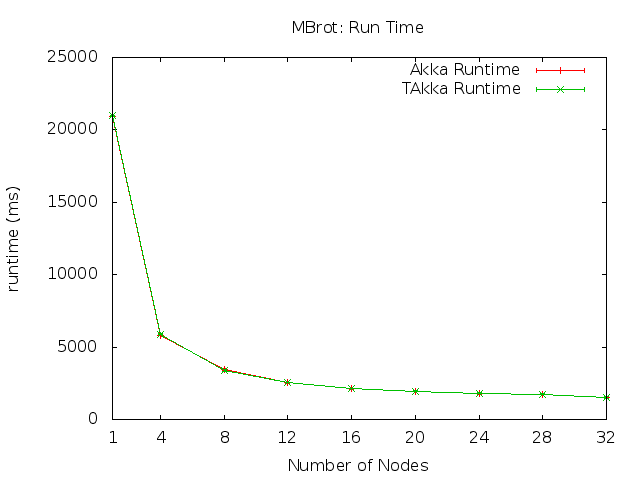
\includegraphics[scale=0.31]{efficiency/MBrot_time.png}
        }
        \subfloat[MBrot6000 Scalability]{
           \label{fig:1v}
           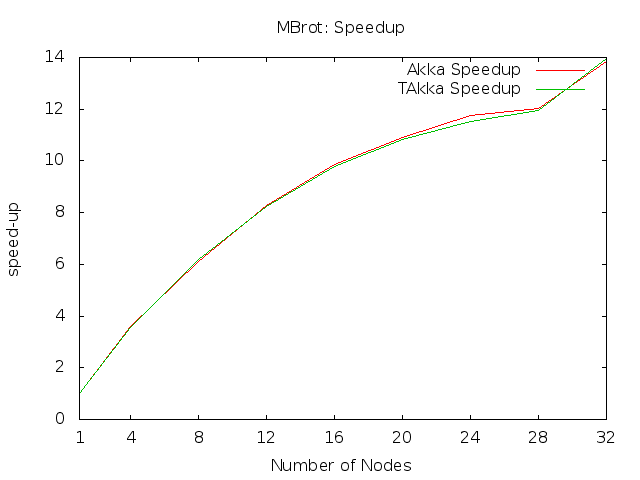
\includegraphics[scale=0.31]{efficiency/MBrot_speedup.png}
        }\\
    \end{center}
    \caption{Benchmark: MBrot}
   \label{mbrot_efficiency}
\end{figure}

The result of the Fibonacci benchmark provides evidence that the scalability
of a distributed application can be bounded by the throughput of the master node.
The same conclusion is obtained when the image size of the MBrot example
is changed.   The MBrot example has a quadratic complexity 
to the image size.  In the BenchErl example, the image size is set to $6000$ 
pixels $ \times$  $ 6000$ pixels so that more time is spent on computation than 
message sending.  Figure~\ref{mbrot_efficiency} reports the results when the 
image size is set to $10$ pixels $ \times$  $ 10$ pixels, $1000$ pixels $ 
\times$  $ 1000$ pixels, and $6000$ pixels $ \times$  $ 6000$ pixels.   As 
expected, the result is similar to the result of the Fibonacci benchmark.  
% The highest speed-up achieved in the MBrot example is smaller than the one in the
% Fibonacci example because each child node in the MBrot example has less computational
% cost.

\subsubsection{The N-Queens Problem}

In the BenchErl examples and the Fibonacci example, child processes are asked to 
execute the same computation a number of times (Section~\ref{bencherl_overview}).  In contrast, distributed and 
cluster computing techniques are often used to solve a computationally 
expensive task by distributing sub-tasks to independent nodes.  To simulate 
such a scenario, another benchmark, N-Queens Puzzle, is added. 

The N-Queen Puzzle \citep{wiki:nqueens} looks for {\it all} solutions of 
placing $n$ queens on an $n \times n$ chessboard such that no two queens share 
the same row, column, or diagonal.  In the benchmark, a master node first uses 
a width-first backtracking algorithm to expand the search space.  If the 
number of candidate partial solutions is greater than twice the available 
nodes, the master node sends partial solutions to those nodes which use a 
depth-first backtracking algorithm to find all possible solutions of each 
candidate partial solution. In this example, two solutions are considered 
distinct if they differ only in symmetry operations.

Finding all solutions of an N-Queen Puzzle is an NP-hard problem.  Therefore, a 
suitable $n$ makes the problem a good benchmark to demonstrate the advantage of 
cluster and distributed programming.  Figure~\ref{nqueens_efficiency}
reports the result when $n$ is set to $14$.  The value of $n$ is chosen 
according to the same criteria for BenchErl benchmarks as stated in Section 
\ref{bench_parameters}.  The result shows that both the Akka and 
TAkka implementation have good scalability and similar efficiency.


\begin{figure}[h]
     \begin{center}
        \subfloat[N-Queens Time]{
            \label{fig:1q}
            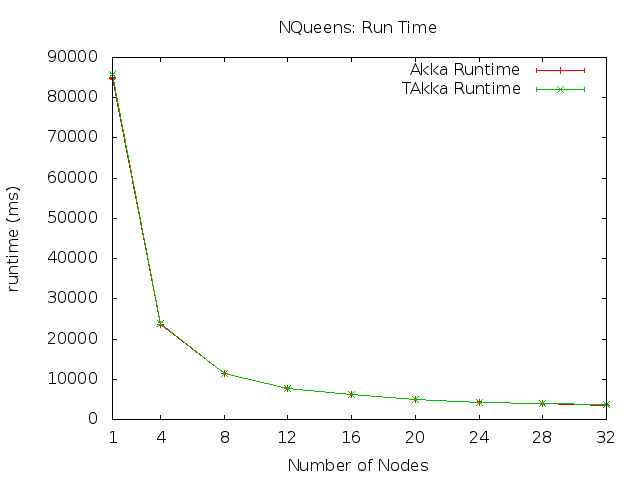
\includegraphics[scale=0.3]{efficiency/NQueens_time.png}
        }
        \subfloat[N-Queens Scalability]{
           \label{fig:1r}
           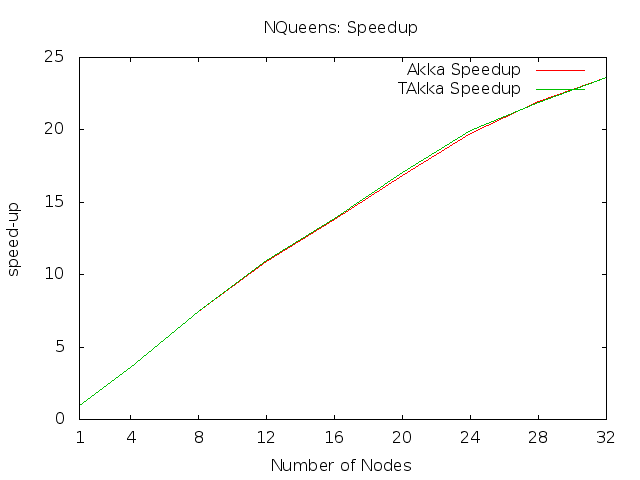
\includegraphics[scale=0.3]{efficiency/NQueens_speedup.png}
        }
    \end{center}
    \caption{Benchmark: N-Queens Puzzle}
   \label{nqueens_efficiency}
\end{figure}



\newpage
\section{Assessing System Reliability and Availability}
\label{reliability}

The supervision tree principle is adopted by Erlang and Akka users in the 
hope of improving the reliability of software applications.  Apart from the 
reported nine "9"s reliability of Ericsson AXD 301 switches 
\citep{ArmstrongAXD} and the wide range of Akka use cases, how could software 
developers assure the reliability of their newly implemented applications?  

TAkka is shipped with a Chaos Monkey library and a Supervision View library for 
assessing the reliability of TAkka applications.  A Chaos Monkey test randomly 
kills actors in a supervision tree and a Supervision View test dynamically 
captures the structure of supervision trees.  With the help of Chaos Monkey and 
Supervision View, users can visualize how their TAkka applications react to 
adverse conditions. Missing nodes in the supervision tree (Section 
\ref{calculator_chaos_test}) show that failures occur during the test. On the 
other hand, any failed actors are restored, and hence appropriately supervised 
applications (Section~\ref{bencherl_chaos_test})  pass Chaos Monkey tests.



\subsection {Chaos Monkey and Supervision View}

Chaos Monkey \citep{ChaosMonkey} randomly kills Amazon Elastic Compute Cloud 
(Amazon EC2) instances in an Auto Scaling Group.  In a Chaos Monkey test, the 
reliability of an application is tested against intensive adverse 
conditions.  The same idea is ported into Erlang to detect potential flaws of 
supervision trees \citep{ErlangChaosMonkey}.  The TAkka library ports the 
Erlang version of Chaos Monkey.  In addition to randomly killing actors, 
users can simulate other common failures by using the following modes.

\paragraph{Random} This is the default mode of Chaos Monkey.  It randomly
choose one of the other modes in each run.

\paragraph{Exception} This mode simulates the case that an exception is raised
from an actor.  The randomly picked victim actor raises an exception from a
user-defined set of exceptions.


\paragraph{Kill} This mode simulates the case that a recoverable failure is occurred
inside an actor.  A {\tt Kill} message is sent to a randomly picked victim actor to see
if it can be restarted by its supervisor.

\paragraph{PoisonKill} This mode simulates that case that an unidentifiable failure
is occurred inside an actor.  A {\tt PoisonKill} message is sent to a randomly
picked victim actor.  The actor is terminated permanently and cannot be restarted
by its supervisor.  It tests whether the application has other failure recovery
mechanism for that actor.  Being supervised is sufficient for most actors.  However,
for some critical actors, having additional assurance might be required in practice.

\paragraph{NonTerminate} This mode simulates network congestion or a design flow of
actor implementation.  A randomly picked actor runs into an infinite loop and
consumes system resources but cannot process any messages.  A robust system should be
able to detect such flow or network congestion, redirect further messages to a new
actor, and try to kill the problematic actor.

\begin{comment}

\begin{table}[h]
\begin{center}
\begin{tabular}{| c | p{4.6 cm} | p{5.2 cm} | }
\hline
Mode & Failure & Description \\
\hline
Random (Default) & Random Failures & Randomly choose one of the other modes in 
each run. \\
\hline
Exception & Raise an exception & A victim actor randomly raise an exception 
from 
a user-defined set of exceptions. \\
\hline
Kill & Failures that can be recovered by scheduling service restart &  
Terminate 
a victim actor.  The victim actor can be restarted later. \\
\hline
PoisonKill & Unidentifiable failures & Permanently terminate a victim actor.  
The victim cannot be restarted.  \\ 
\hline 
NonTerminate & Design flaw or network congestion & Let a victim actor run 
into an infinite loop.  The victim actor consumes system resources but cannot 
process any messages. \\
\hline

\end{tabular}
\caption{TAkka Chaos Monkey Modes}
\label{chaos}
\end{center}
\end{table}

\end{comment}

Figure~\ref{chaos_api} gives the API and the core implementation of TAkka Chaos 
Monkey.  A user sets up a Chaos Monkey test by initializing a 
{\tt ChaosMonkey} instance, defining the test mode, and scheduling the interval 
between each run.  In each run, the {\tt ChaosMonkey} instance sends a 
randomly picked actor a special message.  Upon receiving a Chaos Monkey 
message, a TAkka actor executes a piece of problematic code as described above.  
{\tt PoisonPill} and {\tt Kill} are handled by {\tt 
systemMessageHandler} and can be overridden (Figure~\ref{takka_actor_api}).  
{\tt ChaosException} and {\tt ChaosNonTerminate}, on the 
other hand, are handled by the TAkka library and cannot be overridden.

\begin{figure}[p]

\begin{lstlisting}
package takka.chaos
class ChaosMonkey(victims:List[ActorRef[_]], exceptions:List[Exception]){
  private var status:Status = OFF;
  def setMode(mode:ChaosMode);
  def enableDebug();
  def disableDebug();
  def start(interval:FiniteDuration)  = status match {
    case ON => 
throw new Exception("ChaosMonkey is running: turn it off before restart it.") 
    case OFF =>
      status = ON
      scala.concurrent.future {
        repeat(interval)
      }
  }
  def turnOff()= {status = OFF}
  private def once() {
    var tempMode = mode
    if (tempMode == Random){
      tempMode = Random.shuffle(
                 ChaosMode.values.-(Random).toList).head
    }
    val victim = scala.util.Random.shuffle(victims).head
    tempMode match {
      case PoisonKill =>
        victim.untypedRef ! akka.actor.PoisonPill
      case Kill =>
        victim.untypedRef ! akka.actor.Kill
      case Exception =>
        val e = scala.util.Random.shuffle(exceptions).head
        victim.untypedRef ! ChaosException(e)
      case NonTerminate =>
        victim.untypedRef ! ChaosNonTerminate   
  } }
  private def repeat(period:FiniteDuration):Unit =  status match {
    case ON =>
      once
      Thread.sleep(period.toMillis)
      repeat(period)      
    case OFF =>
} } 
object ChaosMode extends Enumeration {
    type ChaosMode = Value
    val Random, PoisonKill, Kill, Exception, NonTerminate  = Value
}
\end{lstlisting}
\caption{TAkka Chaos Monkey}
\label{chaos_api}
\end{figure}


\subsection{Supervision View}


To dynamically monitor changes in supervision trees, the author designed and 
implemented a Supervision View library. In a supervision view test, an instance 
of {\tt ViewMaster} periodically sends request messages to interested actors.  
When the request message is received, an active TAkka actor replies its 
status to the {\tt ViewMaster} instance and passes the request message to its 
children.  The status message includes its actor path, paths of its children, 
and the time when the reply is sent.  The {\tt ViewMaster} instance records 
status messages and passes them to a visualizer, which will analyze and 
interpret changes in the tree structure during the testing period.


A view master is initialized by calling one of the apply methods of the {\tt 
ViewMaster} object as given in Figure~\ref{supervision_view}.
Each view master has an actor system and a master actor as its fields.  The 
actor system is set up according to the given {\tt name} and {\tt config}, or 
the default configuration.  The master actor, created in the actor system, has 
type {\tt Actor[SupervisionViewMessage]}.  After the start method of a 
view master is called, the view master periodically sends {\tt 
SupervisionViewRequest} to interested nodes in supervision trees, where 
{\tt date} is the system time just before the view master sends requests.  
When a TAkka actor receives {\tt SupervisionViewRequest} message, it sends a 
{\tt SupervisionViewResponse} message back to the view master and passes the \\ 
{\tt SupervisionViewRequest} message to its children.  The {\tt date} value
in a \\ {\tt SupervisionViewResponse} message is the same as the {\tt date} 
value 
in the corresponding {\tt SupervisionViewRequest} message.  Finally, the master 
actor of the view master records all replies in a hash map from {\tt Date} to 
{\tt TreeSet[NodeRecord]}, and sends the record to an appropriate drawer on 
request. 



\begin{figure}[!h]

\begin{lstlisting}
package takka.supervisionview
sealed trait SupervisionViewMessage
case class SupervisionViewResponse(date:Date, reportorPath:ActorPath, 
    childrenPath:List[ActorPath]) extends SupervisionViewMessage
case class ReportViewTo
    (drawer:ActorRef[Map[Date, TreeSet[NodeRecord]]]) 
    extends SupervisionViewMessage

case class SupervisionViewRequest(date:Date,  
              master:ActorRef[SupervisionViewResponse])
case class NodeRecord(receiveTime:Date, node:ActorPath, 
              childrenPath:List[ActorPath]) 

object ViewMaster{
  def apply(name:String, config: Config, topnodes:List[ActorRef[_]], 
              interval:FiniteDuration):ViewMaster
  
  def apply(name:String, topnodes:List[ActorRef[_]], 
              interval:FiniteDuration):ViewMaster
  
  def apply(topnodes:List[ActorRef[_]], 
              interval:FiniteDuration):ViewMaster
}


\end{lstlisting}
\caption{Supervision View}
\label{supervision_view}
\end{figure}

\begin{figure}[p]
     \begin{center}
        \subfloat[]{
            \label{fig:tree1}
            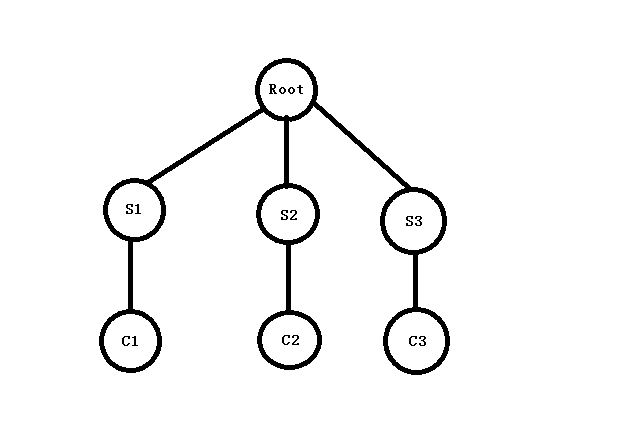
\includegraphics[scale=0.6]{Tree1.png}
        }\\
        \subfloat[]{
           \label{fig:tree2}
           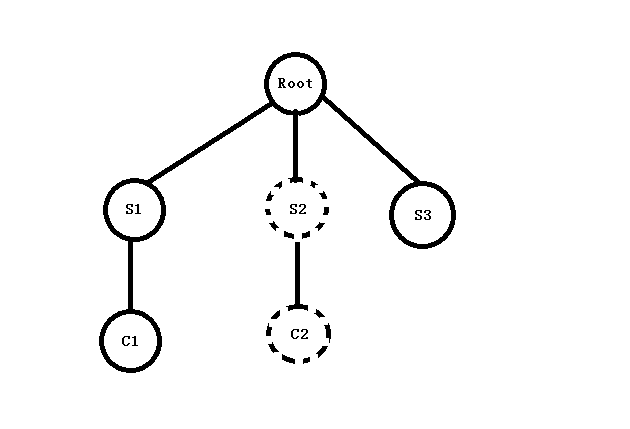
\includegraphics[scale=0.6]{Tree2.png}
        }\\
        \subfloat[]{
            \label{fig:tree3}
            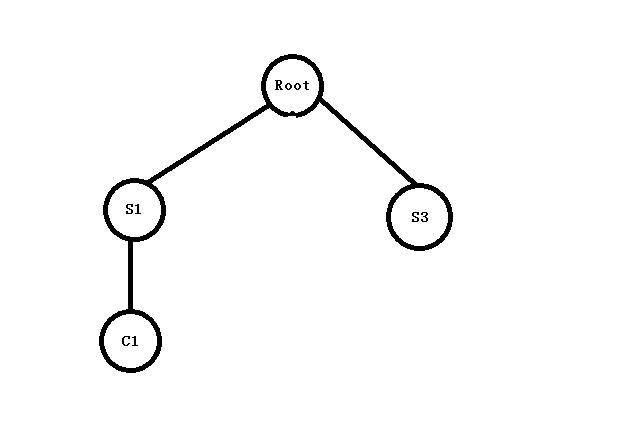
\includegraphics[scale=0.6]{Tree3.png}
        }
    \end{center}
    \caption{Supervision View Example}
   \label{fig:supervisionview}
\end{figure}

\subsection{A Partly Failed Safe Calculator}
\label{calculator_chaos_test}

In the hope that Chaos Monkey and Supervision View tests could reveal 
the breaking points in a supervision tree, the author modified the Safe 
Calculator example and ran a test as follows.  Firstly, three 
safe calculators were run on three Beowulf nodes, under the supervision of a 
root actor using the {\tt OneForOne} strategy with {\tt Restart} action.  
Secondly, different supervisor strategies were set for each safe calculator.  
The first safe calculator, S1, restarts any failed child immediately.  This 
configuration simulates a quick restart process. The second safe calculator, 
S2, computes a Fibonacci number in a naive way for about 10 seconds before 
restarting any failed child.  This configuration simulates 
a restart process which may take a noticeable time.  The third safe calculator, 
S3, stops the child when it fails.  Finally, a Supervision View test was set to 
capture the supervision tree every 15 seconds, and a Chaos Monkey 
test was set to kill a random child calculator every 3 seconds.

A test result, given in Figure~\ref{fig:supervisionview}, gives the expected
tree structure at the beginning, 15 seconds and 30 seconds of the test.  Figure 
\ref{fig:tree1} shows that the application initialized three safe calculators 
as described.  In Figure~\ref{fig:tree2}, S2 and its child are marked as dashed 
circles because it takes the view master more than 5 seconds to receive their 
responses.  From the test result itself, a user cannot tell whether the delay 
is due to a blocked calculation or network congestion.  Comparing against 
Figure~\ref{fig:tree1}, the child of S3 is not shown in Figure~\ref{fig:tree2} 
and Figure~\ref{fig:tree3} because no response is received from it until the 
end of the test.  When the test ends, no response to the last request is 
received from S2 and its child.  Therefore, both S2 and its child are not shown 
in Figure~\ref{fig:tree3}.  S1 and its child appear in all three Figures 
because either they never fail during the test or they are recovered from 
failures within a short time.




\subsection{BenchErl Examples with Different Supervisor Strategies}
\label{bencherl_chaos_test}

To test the behaviour of applications with internal states under 
different supervisor strategies, the author applied the {\tt OneForOne} 
supervisor strategy with different {\tt Directive}s (Figure~\ref{takka_supervisor_strategy}) to the 8 BenchErl examples 
and tested them using Chaos Monkey and Supervision View.  The master node of 
each BenchErl test was initialized with an internal counter.  The internal 
counter decreased when the master node received finishing messages from its 
children.  The test application stopped when the internal counter of the master 
node reached 0.  The Chaos Monkey test is set with the {\tt Kill} mode 
and randomly killed a victim actor every second.  When the {\tt Escalate} 
directive is applied to the master node, the test stops as soon as the first {\tt 
Kill} message is sent from the Chaos Monkey test.  When the {\tt Stop} directive 
is applied, the application does not stop and, eventually, the supervision view 
test only receives messages from the master node.  When the {\tt Restart} 
directive is applied, the application does not stop but the Supervision View test 
receives messages from the master node and its children.  When the {\tt Resume} 
directive is applied, all tests stop eventually with a longer run-time compared to 
tests without Chaos Monkey and Supervision View.



\begin{comment}
\subsubsection{Limitation of Accelerated Software Reliability Test}

By following the Supervision Principle, software developers hope their 
applications can be tolerant of run-time exceptions.
\end{comment}

\section{Summing Up}

This chapter confirms that TAkka can detect type errors without bringing in 
obvious overheads.  Firstly, all small and medium sized Akka examples used in 
this chapter are straightforwardly rewritten using the TAkka library, by 
updating about 7.4\% of the source code.  Through the porting process, a type 
error was found in the Socko framework.  The case study in Section 
\ref{takka_evaluation} shows that TAkka has the 
advantage of solving the type pollution problem.  Secondly, web 
servers built using Akka and TAkka reach similar throughput when the same 
number of EC2 instances are used.  Thirdly, BenchErl benchmark examples written 
in Akka and TAkka have similar efficiency and scalability when running on a 
32 node Beowulf cluster.  The additional benchmark examples in Section 
\ref{bench_fib} provide evidences that the scalability of an application 
depends on the ratio of the cost of parallelized computational tasks and the 
cost of throughput bounded communications.  Lastly, TAkka provides a ChaosMonkey 
library and a Supervision View library for assessing the correctness of 
applications built using TAkka. 


